\chapter{Multiresolution Sinusoidal Neural Networks}
\label{chap:mr_snn}

In this chapter, we present a novel family of neural network architectures designed to efficiently encode signals at multiple scales. Our objective is to construct a continuous, compact, and high-fidelity representation of scalar and vector fields, making it applicable to a variety of media such as audio, images, shapes, and complex spatiotemporal data. These media object, interpreted as signals, can be given explicitly as attributes of space-time coordinates or implicitly as level sets of functions.

This chapter builds upon our exploration of sinusoidal neural networks, where we analyzed how frequency capacity and initialization schemes influence the network's ability to represent diverse signal frequencies. Drawing on these insights, we propose a multiresolution neural network (MR-Net) architecture that combines classical multi-scale signal processing techniques with modern deep learning methodologies to address the limitations of existing coordinate-based models.

The MR-Net framework introduces a unified architecture capable of encoding signals in a multiscale manner, supporting flexible training regimes and progressive refinement. It includes three primary subclasses, each designed for distinct frequency control scenarios: \emph{S-Net}, \emph{L-Net}, and \emph{M-Net}. These subclasses offer different trade-offs between frequency resolution and control, and computational efficiency, providing a versatile toolkit for representing complex signals across a range of applications.

To implement the multiresolution approach, we draw inspiration from classical signal processing techniques such as Gaussian and Laplacian pyramids. In MR-Net, levels of detail are determined by spectral projections, and training proceeds in a progressive manner, refining the representation incrementally. The preliminary versions of MR-Net were first presented in \cite{paz2022,paz2023mr}. In the following sections, we describe the theoretical foundations, design principles, and architectural details of MR-Net, providing a comprehensive overview of the framework and its potential applications.

% Key features of the MR-Net framework include:

% \begin{itemize}
%     \item \textbf{Flexible Data Handling}: MR-Net can be trained with various types of data, including regularly sampled grids, hierarchical multiresolution structures such as pyramids, or through stochastic and stratified sampling.
%     \item \textbf{Adaptive Level of Detail}: The network can adapt its representation to match the input data's resolution. For multiresolution training, levels of detail are determined by spectral projections, while for single-resolution inputs, they are governed by the network's capacity and initialization control.
%     \item \textbf{Progressive Training Paradigms}: Training proceeds in a progressive manner, refining the representation incrementally. This approach ensures efficient learning across a range of scales and improves convergence for high-frequency details.
%     \item \textbf{Continuous Multiscale Representation}: The MR-Net architecture encodes signals in a continuous manner, both in spatial and scale dimensions, enabling seamless reconstruction at arbitrary resolutions.
% \end{itemize}

% For the multiresolution approach, we leverage classical structures of image and signal processing, such as Gaussian and Laplacian Pyramids. We use these ideas to develop a framework to train a multi-stage neural network using multiresolution structures in an efficient way. \red{Finally, we demonstrate that our model can achieve a comparable reconstruction quality to a simple SIREN model with the same number of parameters, while encoding multiple levels of detail. Esta frase deve ser movida para o capítulo seguinte, de aplicações em imagens. A conclusão desta parte será finalizada quando este capítulo estiver completo.}

% \red{We have established that we can bound the frequencies learned by a sinusoidal neural network by adjusting the interval of frequencies sampled for initialization of its first layer, and also by adjusting the network capacity. That is, if the value of $\omega_0$ is too low, the network will learn the lower frequencies of the signal, fitting their intensities in the Fourier spectrum, but won't learn the higher frequencies, even if it has enough computational units to to do. On the other hand, if the capacity given by the computational units is too small, the result will also resemble a filtered version of the target signal. TALVEZ MOVER PARA O CHAPTER 4 - MR-TRAINING}

\section{Related Works}

Multiresolution analysis has its roots in the seminal work of (\cite{mallat1989theory}) and (\cite{daubechies92}), who formalized the wavelet transform as a powerful tool for analyzing signals at different scales. Their contributions provided the framework for decomposing signals into distinct frequency bands while preserving spatial or temporal information, which is essential for many signal processing applications.

Integrating multiresolution concepts with neural network architectures has led to several innovative developments. One such approach is the scattering networks proposed by \citet{bruna2013}, which apply cascaded wavelet transforms followed by nonlinear operators to produce stable, translation-invariant signal representations. For image-related tasks, architectures such as those by \citet{sppHe2015} and \citet{YuKoltun2016} employ Convolutional Neural Networks (CNNs) to process inputs at multiple scales simultaneously. However, these models are primarily designed to extract features from large datasets for applications such as image classification, rather than to represent signals in a multiresolution format.

\citet{zhangWavelet92} introduced Wavelet Neural Networks (WNNs), which leverage wavelet functions as activation units, replacing traditional perceptrons with \textit{wavelons} to perform adaptive wavelet transforms on input signals. While WNNs offer a novel alternative to perceptron-based neural networks, some inherent limitations might have prevented further development on this approach. First, unlike deep neural networks that learn hierarchical features, WNNs architectures are shallow and, thus, require a significantly larger number of parameters to achieve high-fidelity signal representation. Furthermore, WNNs can be challenging to optimize, with their performance heavily influenced by the initial choice of wavelet functions and corresponding parameters.

In the domain of coordinate-based neural networks, \citet{bacon2021} introduced the Band-Limited Coordinate Network (BACON), which is built on the Multiplicative Filter Network architecture \citep{fathony2020multiplicative}. BACON generates intermediate outputs with predefined spectral bandwidth, achieving multiresolution representations of underlying signals. While its structure allows BACON to be expressed as a linear combinations of sines, avoiding the composition of sines present in deep sinusoidal MLPs, it creates multiresolution representations by truncating the frequency spectra of the signals at a specific value. This method introduces ringing artifacts at certain levels of detail, as evident in the Fourier transforms of images reconstructed using BACON (see Chapter \ref{ch:imaging}).

% The ability to control frequency bands in representation is closely tied to the capability of adaptively reconstructing signals at multiple levels of detail. \citet{mueller2022instant} developed a multiresolution neural network architecture based on hash encoding, while \citet{martel2021acorn} designed an adaptive coordinate network for neural signals.

Frequency band control is crucial for adaptively reconstructing signals across multiple levels of detail. Recent works have explored this idea: \citet{mueller2022instant} presented a multiresolution neural network based on hash encoding, and \citet{martel2021acorn} proposed ACORN, an adaptive coordinate network for representing neural signals. \red{HOW AM I DIFFERENT OF THESE WORKS????? A LITTLE BIT OF TEXT HERE TO ACT AS A PLACEHOLDER UNTIL I HAVE A SATISFACTORY ANSWER TO THIS QUESTION TO PUT IN THIS DISSERTATION.}

In this context, we introduce \textit{Multiresolution Sinusoidal Neural Networks} (MR-Net) \citep{paz2022,paz2023mr} based on classical signal multiresolution representations. Our results in imaging applications, discussed in Chapter \ref{ch:imaging}, demonstrate that MR-Net outperforms the previous state-of-the-art technique, BACON, while utilizing a smaller number of parameters.


% # Weaknesses of Wavelet Neural Networks

% ## 1. Training Complexity

% - WNNs often require optimization of wavelet parameters (scaling and translation) along with the usual network weights.
% - This increases the number of parameters to be learned, potentially leading to longer training times and increased risk of overfitting.
% - The optimization landscape can be more complex, with many local minima, making it challenging to find optimal solutions.

% ## 2. Limited Representational Capacity

% - While effective for certain types of signals, WNNs may struggle with very complex or high-dimensional data.
% - The fixed wavelet basis might not be optimal for all types of signals or tasks.
% - Compared to modern deep learning architectures, WNNs often have lower representational capacity, limiting their performance on complex tasks.

% ## 3. Lack of Hierarchical Feature Learning

% - Unlike deep neural networks that learn hierarchical features, WNNs typically have a shallow architecture.
% - This can limit their ability to capture complex, multi-level abstractions in the data.
% - The absence of multiple layers of nonlinear transformations can restrict the network's ability to learn intricate patterns.

% ## 4. Sensitivity to Initial Conditions

% - The performance of WNNs can be highly dependent on the initial choice of wavelet functions and their parameters.
% - Poor initialization can lead to suboptimal results or slow convergence during training.

% ## 5. Limited Adaptability

% - Once trained, the wavelet basis in WNNs is fixed, which can limit their adaptability to new, unseen data.
% - This contrasts with some modern architectures that can adapt their feature extraction process more flexibly.


\section{Multiscale Representation and Learning}
% Título Alternativo "Multiresolution Signal Decomposition"
\label{s-motivation}


Let $\gt{f}:\mathcal{D}\to \mathcal{C}$ be a \textit{ground-truth signal}, where $\mathcal{D}$ and $\mathcal{C}$ are finite-dimensional vector spaces representing the signal's domain and codomain, respectively. For instance, to represent an image, $\mathcal{D}$ can be set to $\R^2$ to define the spatial domain, while $\mathcal{C}=\R^3$ corresponds to the RGB color space. Throughout this text, we use a cursive font to denote ground-truth signals and a standard font for their corresponding neural network approximations.

To represent the signal $\gt{f}$ at multiple scales, we decompose it into a sum of $N$ stages: $\gt{f}=\gt{g}_0+\dots+\gt{g}_{N-1}$, where $\gt{g}_0$ captures the coarsest approximation of the signal and $\gt{g}_i$, for $i>0$, progressively introduce higher frequency components. This multiresolution decomposition enables us to define the \textit{level of detail}~$i$ in two equivalent forms:

\begin{equation}
\gt{f}_i = \gt{g}_0 + \cdots + \gt{g}_i \quad \text{or} \quad \gt{f}_i = \gt{f} - \sum_{j=i+1}^{N-1} \gt{g}_j.
\end{equation}

Each stage $\gt{g}_i$ can be computed as:
\begin{equation}
\gt{g}_i = \gt{f}_{i+1} - K * \gt{f}_{i+1}, \quad \text{where } \gt{f}_{N-1} = \gt{f}.
\end{equation}

That is, each stage $\gt{g}_i$ represents the difference between the $(i+1)$-th level and its smoothed version obtained by convolving it with a low-pass filter $K$. For instance, $K$ could be a \textit{Gaussian kernel} defined as $G(x,t)=\frac{1}{2\pi t}\exp{(-\frac{\norm{x}^2}{2t})}$, where $t$ is the scale parameter. This way, the sequences $\{\gt{f}_i\}$ and $\{\gt{g}_i\}$ correspond to the \textit{Gaussian} and \textit{Laplacian pyramids}, which are standard tools in multiresolution analysis of digital images \citep{lindeberg1994scale, velho2009image, rosenfeld2013multiresolution}.

Given this multiscale decomposition, our goal is to represent a signal $\gt{f}$ using a family of sinusoidal neural networks. Motivated by the hierarchical structure of $\gt{f}=\gt{g}_0+\dots+\gt{g}_{N-1}$, we propose an aggregation of $N$ sinusoidal MLPs, denoted by $g_i:\mathcal{D}\to \mathcal{C}$, to approximate each stage $\gt{g}_i$. By training each $g_i$ to match the corresponding stage $\gt{g}_i$, we gain precise control over the frequency spectrum learned by each network. This approach leverages the spectral bias of sinusoidal networks, as demonstrated in Chapter \ref{chap:sinusoidal}, allowing the network to naturally prioritize lower frequencies and gradually introduce higher-frequency details.

Each network stage $g_i$ is initialized with a specific and crescent range of frequencies, ensuring that the resulting approximation accurately matches the desired stage $\gt{g}_i$. This structured frequency learning enables us to decompose and reconstruct complex signals in a progressive and controlled manner.

\section{MR-Net Architecture}

The MR-Net architecture is a family of continuous multiresolution networks designed to approximate a complex signal by progressively adding details at multiple levels of resolution. The architecture is defined as a function \( f:\mathcal{D} \times [0,N] \to \mathcal{C} \), where \(\mathcal{D}\) and \(\mathcal{C}\) represent the domain and codomain, respectively. Formally, the MR-Net is expressed as follows:

\begin{align}\label{e-mrnet}
f(x,t) = c_0(t) g_0(x) + \cdots + c_{N-1}(t) g_{N-1}(x),
\end{align}

where each function \( g_i : \mathcal{D} \to \mathcal{C} \) is a \textbf{Multiresolution (MR) Module} —a building block of the MR-Net that is defined in detail in Sec~\ref{s-mr-module}. The MR-Net is composed of \( N \) such MR Modules, each corresponding to a different stage in the multiresolution hierarchy of \( f \). 

The contributions of each MR Module \( g_i \) are controlled by a set of blending functions \( c_i(t) \), defined as:

\begin{align}\label{e-control}
c_i(t) = \max \Big\{ 0, \min \big\{ 1, t - i \big\} \Big\}.
\end{align}

Intuitively, this function ensures that:

\begin{itemize}
    \item When \( t < i \), \( c_i(t) = 0 \).
    \item When \( i \leq t \leq i+1 \), \( c_i(t) = t - i \).
    \item When \( t > i + 1 \), \( c_i(t) = 1 \).
\end{itemize}

Therefore, if \( t = k + \delta \) (with \( k \in \mathbb{N} \) and \( 0 \leq \delta \leq 1 \)), we can express \( f(x, t) \) as the linear combination:

\begin{align}
f(x, t) = g_0(x) + \cdots + g_k(x) + \delta \, g_{k+1}(x).
\end{align}

Each stage function \( f_t := f(\cdot, t) : \mathcal{D} \to \mathcal{C} \) defines a \textit{level of detail} parameterized by \( t \). The resulting MR-Net $f$ learns the decomposition of the ground-truth signal $\gt{f}$ as a projection into the coarse scale space and a sequence of finer detail spaces. For instance, the initial stage $f_1=g_0$ provides the least detailed approximation~of~$f_N$. As \( t \) evolves from 0 to \( N \), these stages progressively refine the representation of the signal, with \( f_N = g_0 + \cdots + g_{N-1} \) representing the full-resolution approximation.

To train this architecture, we fit \( f \) to the ground-truth signal \( \gt{f} = \gt{g}_0 + \cdots + \gt{g}_{N-1} \) by initializing and training each stage \( g_i \) to approximate the corresponding stage of the ground-truth decomposition. In Section \ref{s:training}, we provide more details on training.

This structure aligns with the concept of Multiresolution Analysis (\cite{mallat-mr89}), where a function is decomposed into a sequence of approximations and detail spaces, each stage refining the approximation of the original signal. The MR-Net enables a continuous traversal through these stages using the scale parameter \(t\), allowing seamless navigation across multiple resolutions. Fig.~\ref{f:mrnet-arch} shows the general architecture of an MR-Net having \(N\) stages.

\begin{figure}[!h]
\centering
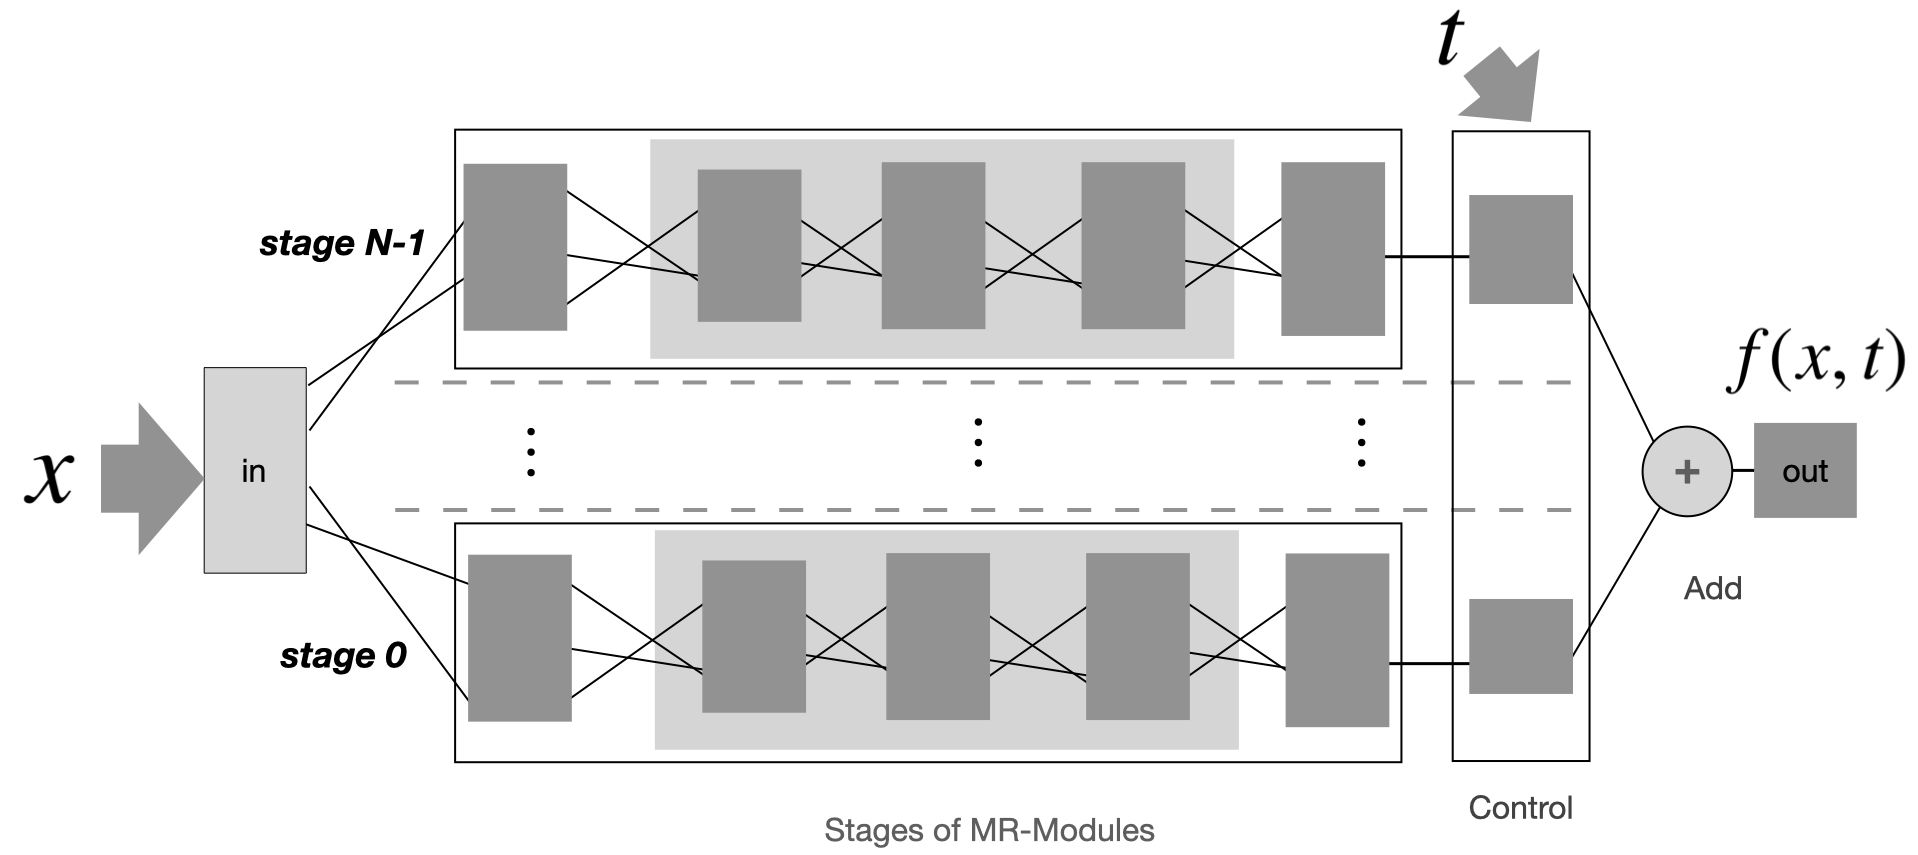
\includegraphics[width=0.9\linewidth]{img/ch4/mr-net-stages-v2.png}
\caption{Anatomy of the MR-Net Family.}
\label{f:mrnet-arch}
\end{figure}


\subsection{MR-Module}
\label{s-mr-module}

Each stage \( g_i \) in the MR-Net is a \textit{Multiresolution (MR) Module}, defined as a sinusoidal MLP with induced frequency bands. A MR-Module is constructed as a function \( g_i = L_i \circ H_i \circ S_i \), illustrated in the Figure \ref{f:mr-module}, where:

\begin{itemize}
    \item \( S_i \): The sinusoidal input layer that projects \( x \in \mathcal{D} \) into a list of sines, generating \( S_i(x) \).
    \item \( H_i \): A sequence of hidden layers (optional), composing \( k \) intermediate transformations of the sines. The output $H_i\circ S_i(x)$ is a dictionary of sine combinations.
    \item \( L_i \): The final linear layer that combines these transformations, the atoms of the dictionary.
\end{itemize}


\begin{figure}[!h]
    \centering
    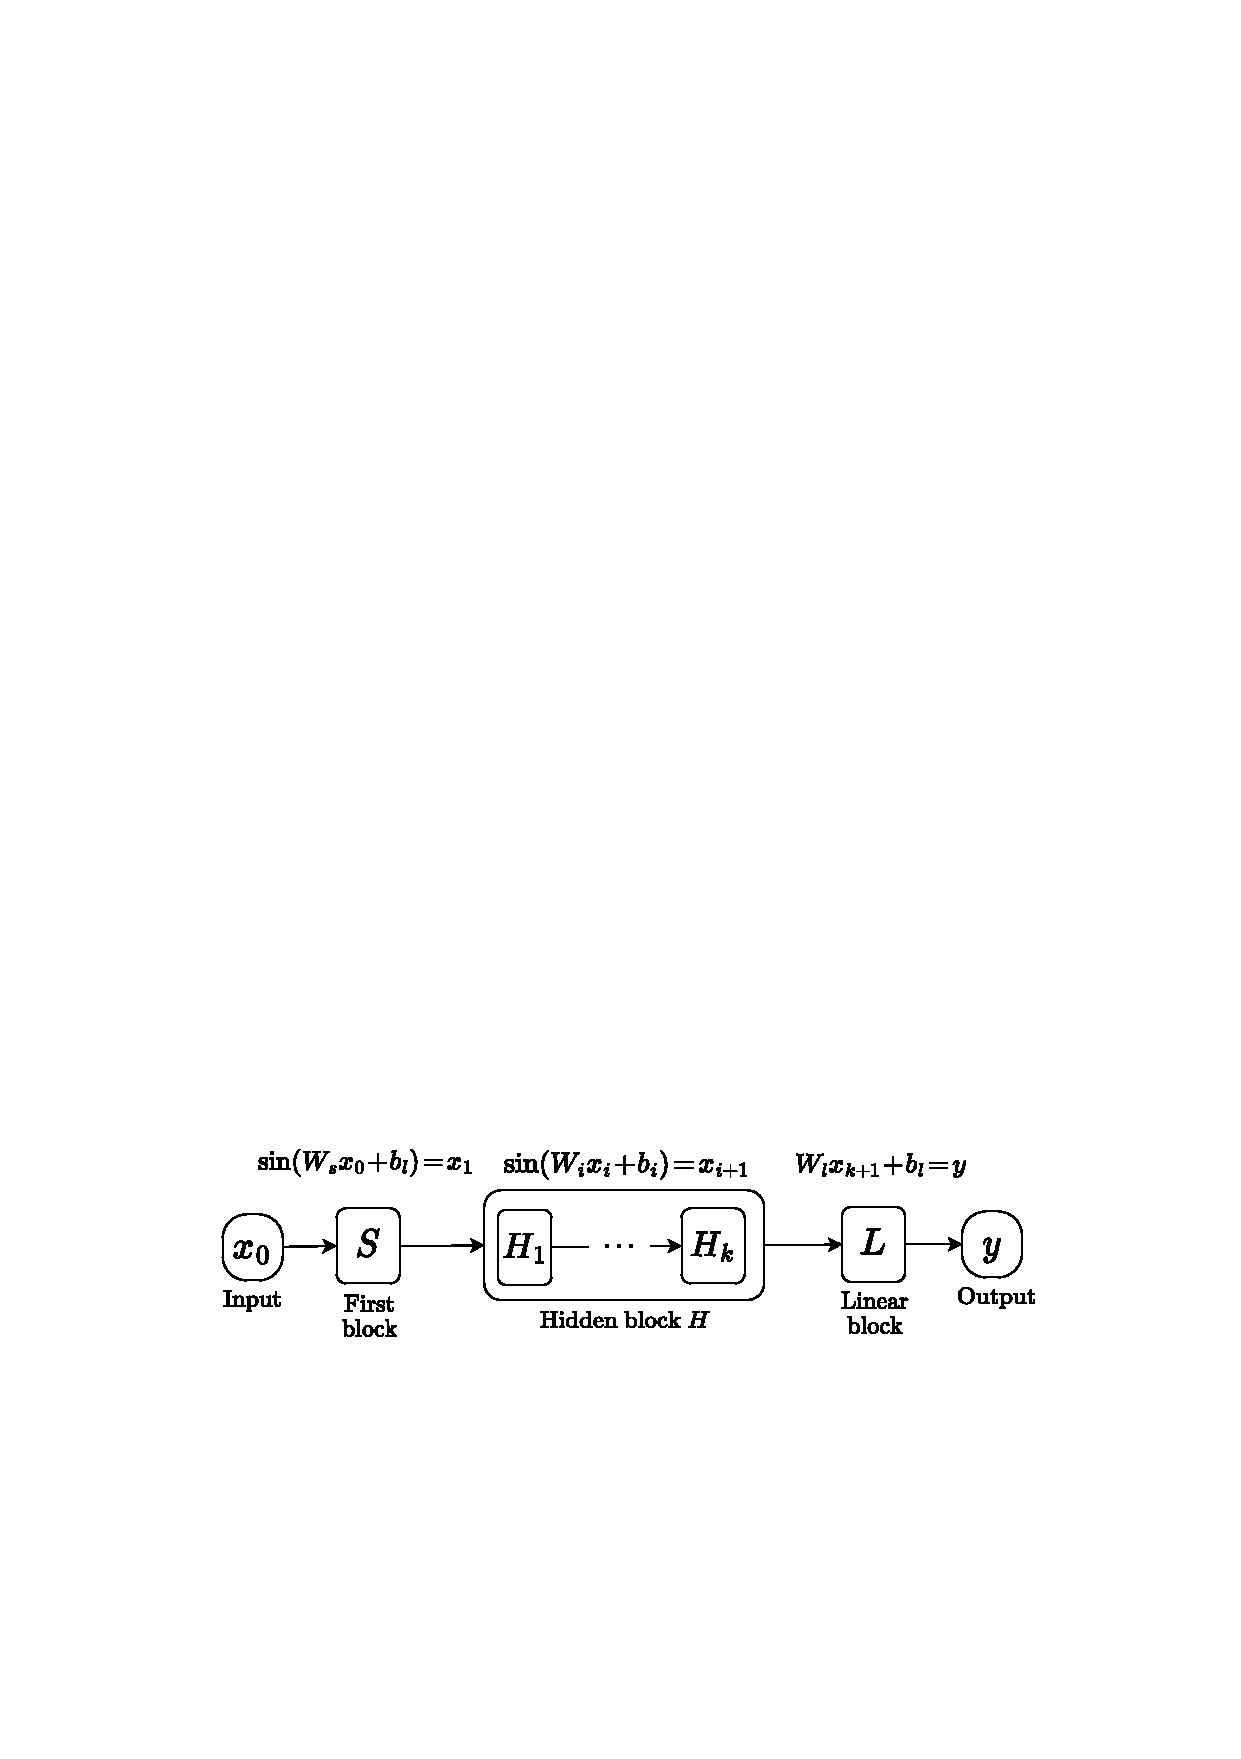
\includegraphics[width=0.9\linewidth]{img/ch4/diagram_mr_module.pdf}
    \caption{General Anatomy of a MR-Module.}
    \label{f:mr-module}
\end{figure}

The specific choice and configuration of these layers define the two types of MR-Modules: \textbf{Pure Sine MR-Module}, a shallow MLP with only the sinusoidal layer \( S \) and linear layer \( L \); and \textbf{Modulated Sine MR-Module}, a deep MLP that includes one or more hidden layers \( H \).

At the end of each level, the control layer \( c_i(t) \) regulates the blending of the MR-Modules, allowing for continuous transitions between stages.

\subsubsection{Pure Sine MR-Module}

The \textit{Pure Sine MR-Module} is a shallow sinusoidal multi-layer perceptron (MLP) that serves as a basic spectral filter. It is defined as the composition \( L \circ S \) of a sinusoidal layer \( S \) followed by a linear output layer \( L \). 

The sinusoidal layer \( S\!:\!\mathbb{R}^d\!\to\! \mathbb{R}^m \) projects the input \( x \in \mathbb{R}^d \) into a dictionary of \( m \) sines of the form \( S(x) = \sin\left(W_s x + b_s\right) \), where \( W_s \in \mathbb{R}^{m \times d} \) is a weight matrix and \( b_s \in \mathbb{R}^m \) is a bias vector. The integer \( m \) is referred to as the \textit{width} of the MR-Module, controlling the number of sinusoidal basis functions used. The linear layer \( L\!:\!\mathbb{R}^m\!\to\! \mathbb{R}^n \) is an affine map defined as \( L(x) = W_l x + b_l \), where \( W_l \in \mathbb{R}^{n \times m} \) and \( b_l \in \mathbb{R}^n \), where $n$ is the dimension of the output vector.

As we saw in Chapter \ref{chap:sinusoidal}, this architecture behaves as a spectral filter because the initialization of \( W_s \) determines the range of frequencies that the MR-Module can capture. Thus, \( W_s \) effectively defines the spectrum of frequencies the module is capable of learning, making it sensitive to the initial configuration of the sine functions.

Figure \ref{f:pure-sine} illustrates the structure of a Pure Sine MR-Module and provides an example of a signal represented as a linear combination of two frequencies. In this example, the sinusoidal layer is defined as \( S(x) = (\sin(x), \sin(5x)) \) and the linear layer simply sums the two outputs, \( L(x_1, x_2) = x_1 + x_2 \).

\begin{figure}[!h]
\centering
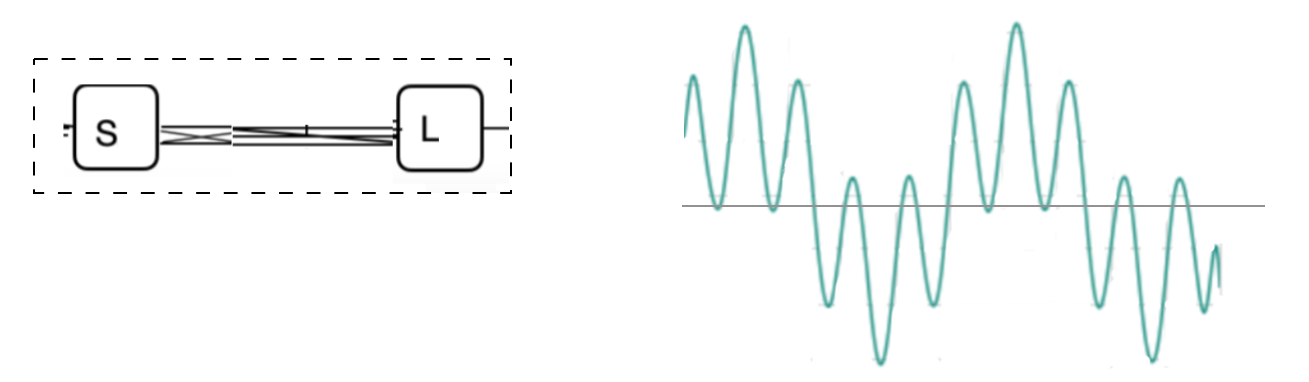
\includegraphics[width=0.8\linewidth]{img/ch4/pure-sine.png}
\caption{Pure Sine MR-Module: Network structure and an example signal formed by a linear combination of two frequencies.}
\label{f:pure-sine}
\end{figure}

\subsubsection{Modulated Sine MR-Module}

The \textit{Modulated Sine MR-Module} extends the capacity of the pure sine version by incorporating additional nonlinear transformations through a deep sinusoidal block. It is defined as a composition \( L \circ H \circ S \), where \( S \) is a sinusoidal layer, \( H \) is a hidden block of multiple sinusoidal transformations, and \( L \) is a linear output layer.

The hidden block \( H\!:\!\mathbb{R}^m\!\to\! \mathbb{R}^m \) is itself a composition of \( k \) sinusoidal layers \( H = H_k \circ \cdots \circ H_1 \), each of the form \( H_i(x_i) = \sin\left(W_i x_i + b_i\right) = x_{i+1} \) for \( i = 1, \dots, k \). Here, \( x_0 \in \mathbb{R}^m \) is the initial input to the hidden block, and the parameters \( m \) and \( k + 1 \) control the \textit{width} and \textit{depth} of the MR-Module. The output layer \( L \!:\! \mathbb{R}^m \!\to\! \mathbb{R}^n \) is similar to the one used in the Pure Sine MR-Module.

This deeper architecture has several implications. First, the Modulated Sine MR-Module has a higher representational capacity than its shallow counterpart for the same number of neurons, due to the hierarchical composition of sine functions \citep{novello2022understanding}. Second, its frequency response is not straightforwardly controlled by the initial weights of \( W_s \), as the nested sinusoidal layers \( H \) create a more complex mapping.

Figure \ref{f:modulated} depicts a Modulated Sine MR-Module and an example of a nested sinusoidal function \( \sin\left( 3\sin\left(5\sin(1.9x)\right)\right) \), showcasing its ability to approximate complex frequency compositions. In this case, the initial sinusoidal layer is \( S(x) = \sin(1.9 x) \), the hidden block is \( H(x) = \sin\left(3\sin(5x)\right) \), and the output layer is simply the identity function \( L(x) = x \). Note that the resulting spectral atoms, i.e., the output functions of \( H \circ S \), can adapt to fit local variations of the input signal's frequencies, enabling a semi-local representation of the signal in both space and frequency domains.

\begin{figure}[!h]
\centering
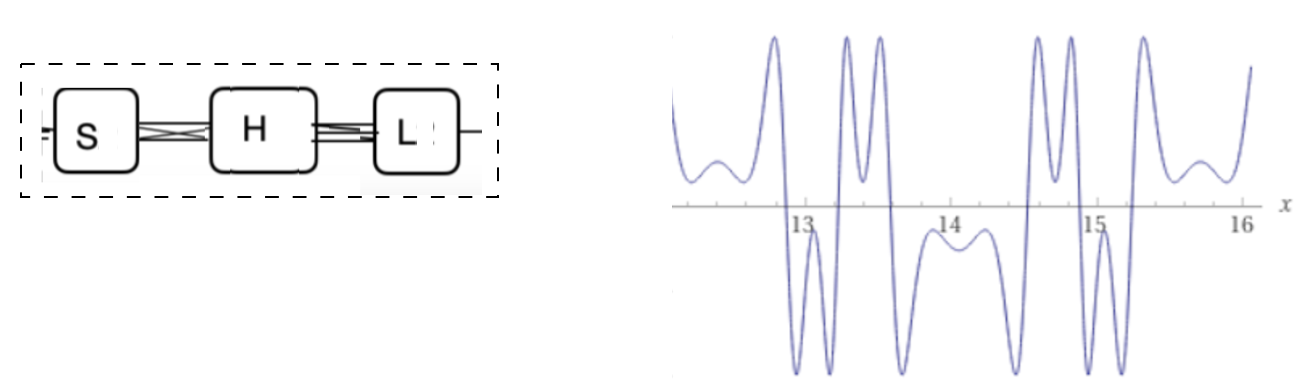
\includegraphics[width=0.9\linewidth]{img/ch4/modulated-sine.png}
\caption{Modulated Sine MR-Module: Network structure and an example of a nested sinusoidal function.}
\label{f:modulated}
\end{figure}

By combining these two types of MR-Modules at different stages of the MR-Net, we can control the approximation of details with varying levels of complexity.

% \red{The choice between *Pure* and *Modulated Sine* modules depends on the desired frequency resolution and localization properties of the signal, making the MR-Net a versatile tool for multiresolution representation.}


\section{MR-Net Subclasses}

In this section, we define three subclasses of the MR-Net, namely, the \textbf{S-Net} (Shallow Network), \textbf{L-Net} (Laplacian Network), and \textbf{M-Net} (Modulated Network), which vary in complexity and representational power depending on the configuration of their stages. Recall from Equation \ref{e-mrnet} that a MR-Net is a function \( f : \mathbb{R}^d \times [0, N] \to \mathbb{R}^n \) defined as a weighted sum of \( N \) individual stages:

\[
f(x, t) = c_0(t)g_0(x) + \cdots + c_{N-1}(t)g_{N-1}(x).
\]

Each stage \( g_i \) corresponds to a neural module that approximates a portion of the target signal at a specific resolution. To specify the subclasses S-Net, L-Net, and M-Net, we configure the internal structure of these stages using different types of sinusoidal MR-Modules, as described below.

\subsection{S-Net: Shallow Sine Stages}

The S-Net is the simplest form of MR-Net, where each stage \( g_i \) is constructed using a pure sine MR-Module. That is, \( g_i = L_i \circ S_i \), where \( S_i \) and \( L_i \) are the first and linear layers, respectively, of the sinusoidal network. Since \( g_i \) is a shallow module, it can be expressed directly as a sum of sine functions:

\begin{align}
    g_i(x) = a_0 + \sum_{j=1}^m a_j \sin\left(\omega_j x + \varphi_j\right),
\end{align}


where the \textit{frequencies} \( \omega_j \) and \textit{phase shifts} \( \varphi_j \) are defined by the weights and biases of the sinusoidal layer \( S_i \). The \textit{amplitudes} \( a_j \) are given by the linear layer \( L_i \).

This structure allows each stage \( g_i \) to serve as a basic spectral filter that captures different frequency components of the input signal. Consequently, the S-Net can control its level of detail by adjusting the frequency bands of each stage. The overall architecture of the S-Net is illustrated in Figure \ref{f:s-net}.

\begin{figure}[!h]
\centering
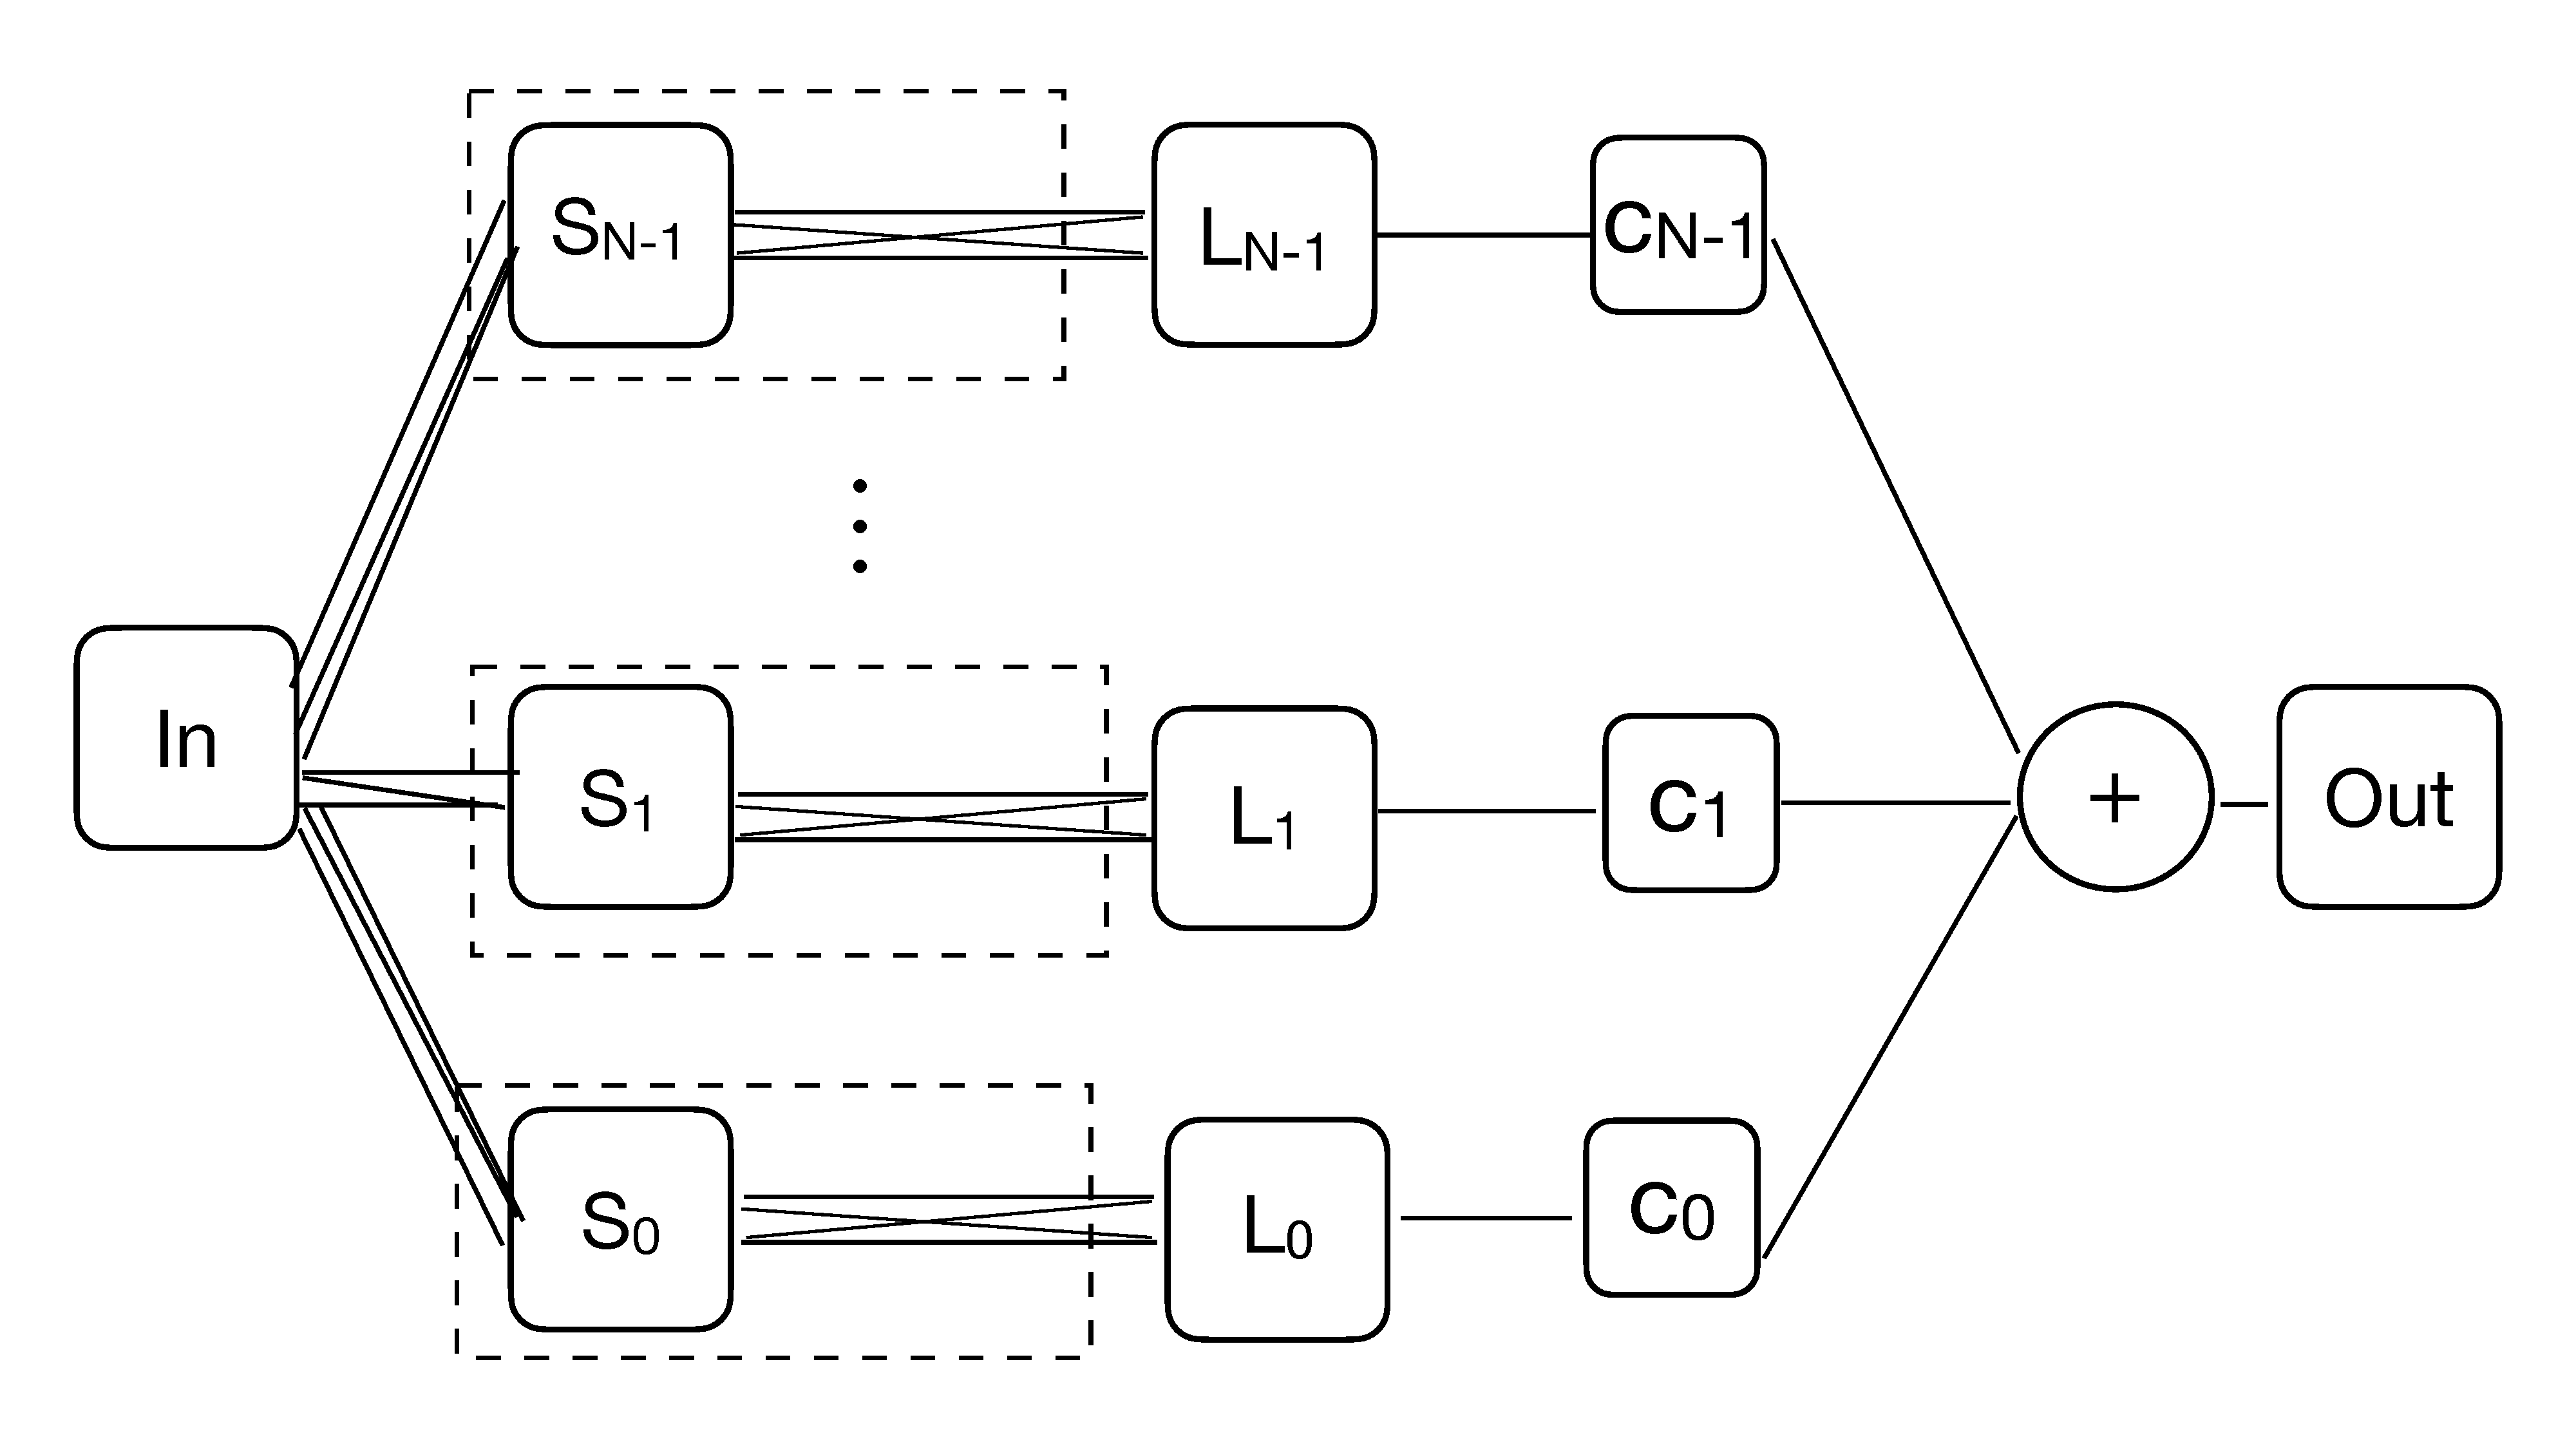
\includegraphics[width=0.58\linewidth]{img/ch4/snet.pdf}
\caption{S-Net architecture: Each stage is a pure sine MR-Module acting as a localized spectral filter.}
\label{f:s-net}
\end{figure}

\subsection{L-Net: Independent Modulated Sine Stages}
\label{s-lnet}

The L-Net extends the S-Net by using a deeper module for each stage \( g_i \). In this configuration, each stage is a modulated sine MR-Module defined as \( g_i = L_i \circ H_i \circ S_i \), where \( S_i \), \( H_i \), and \( L_i \) are the sinusoidal, hidden, and linear layers, respectively (see Fig.~\ref{f:l-net}).

\begin{figure}[!h]
    \centering
    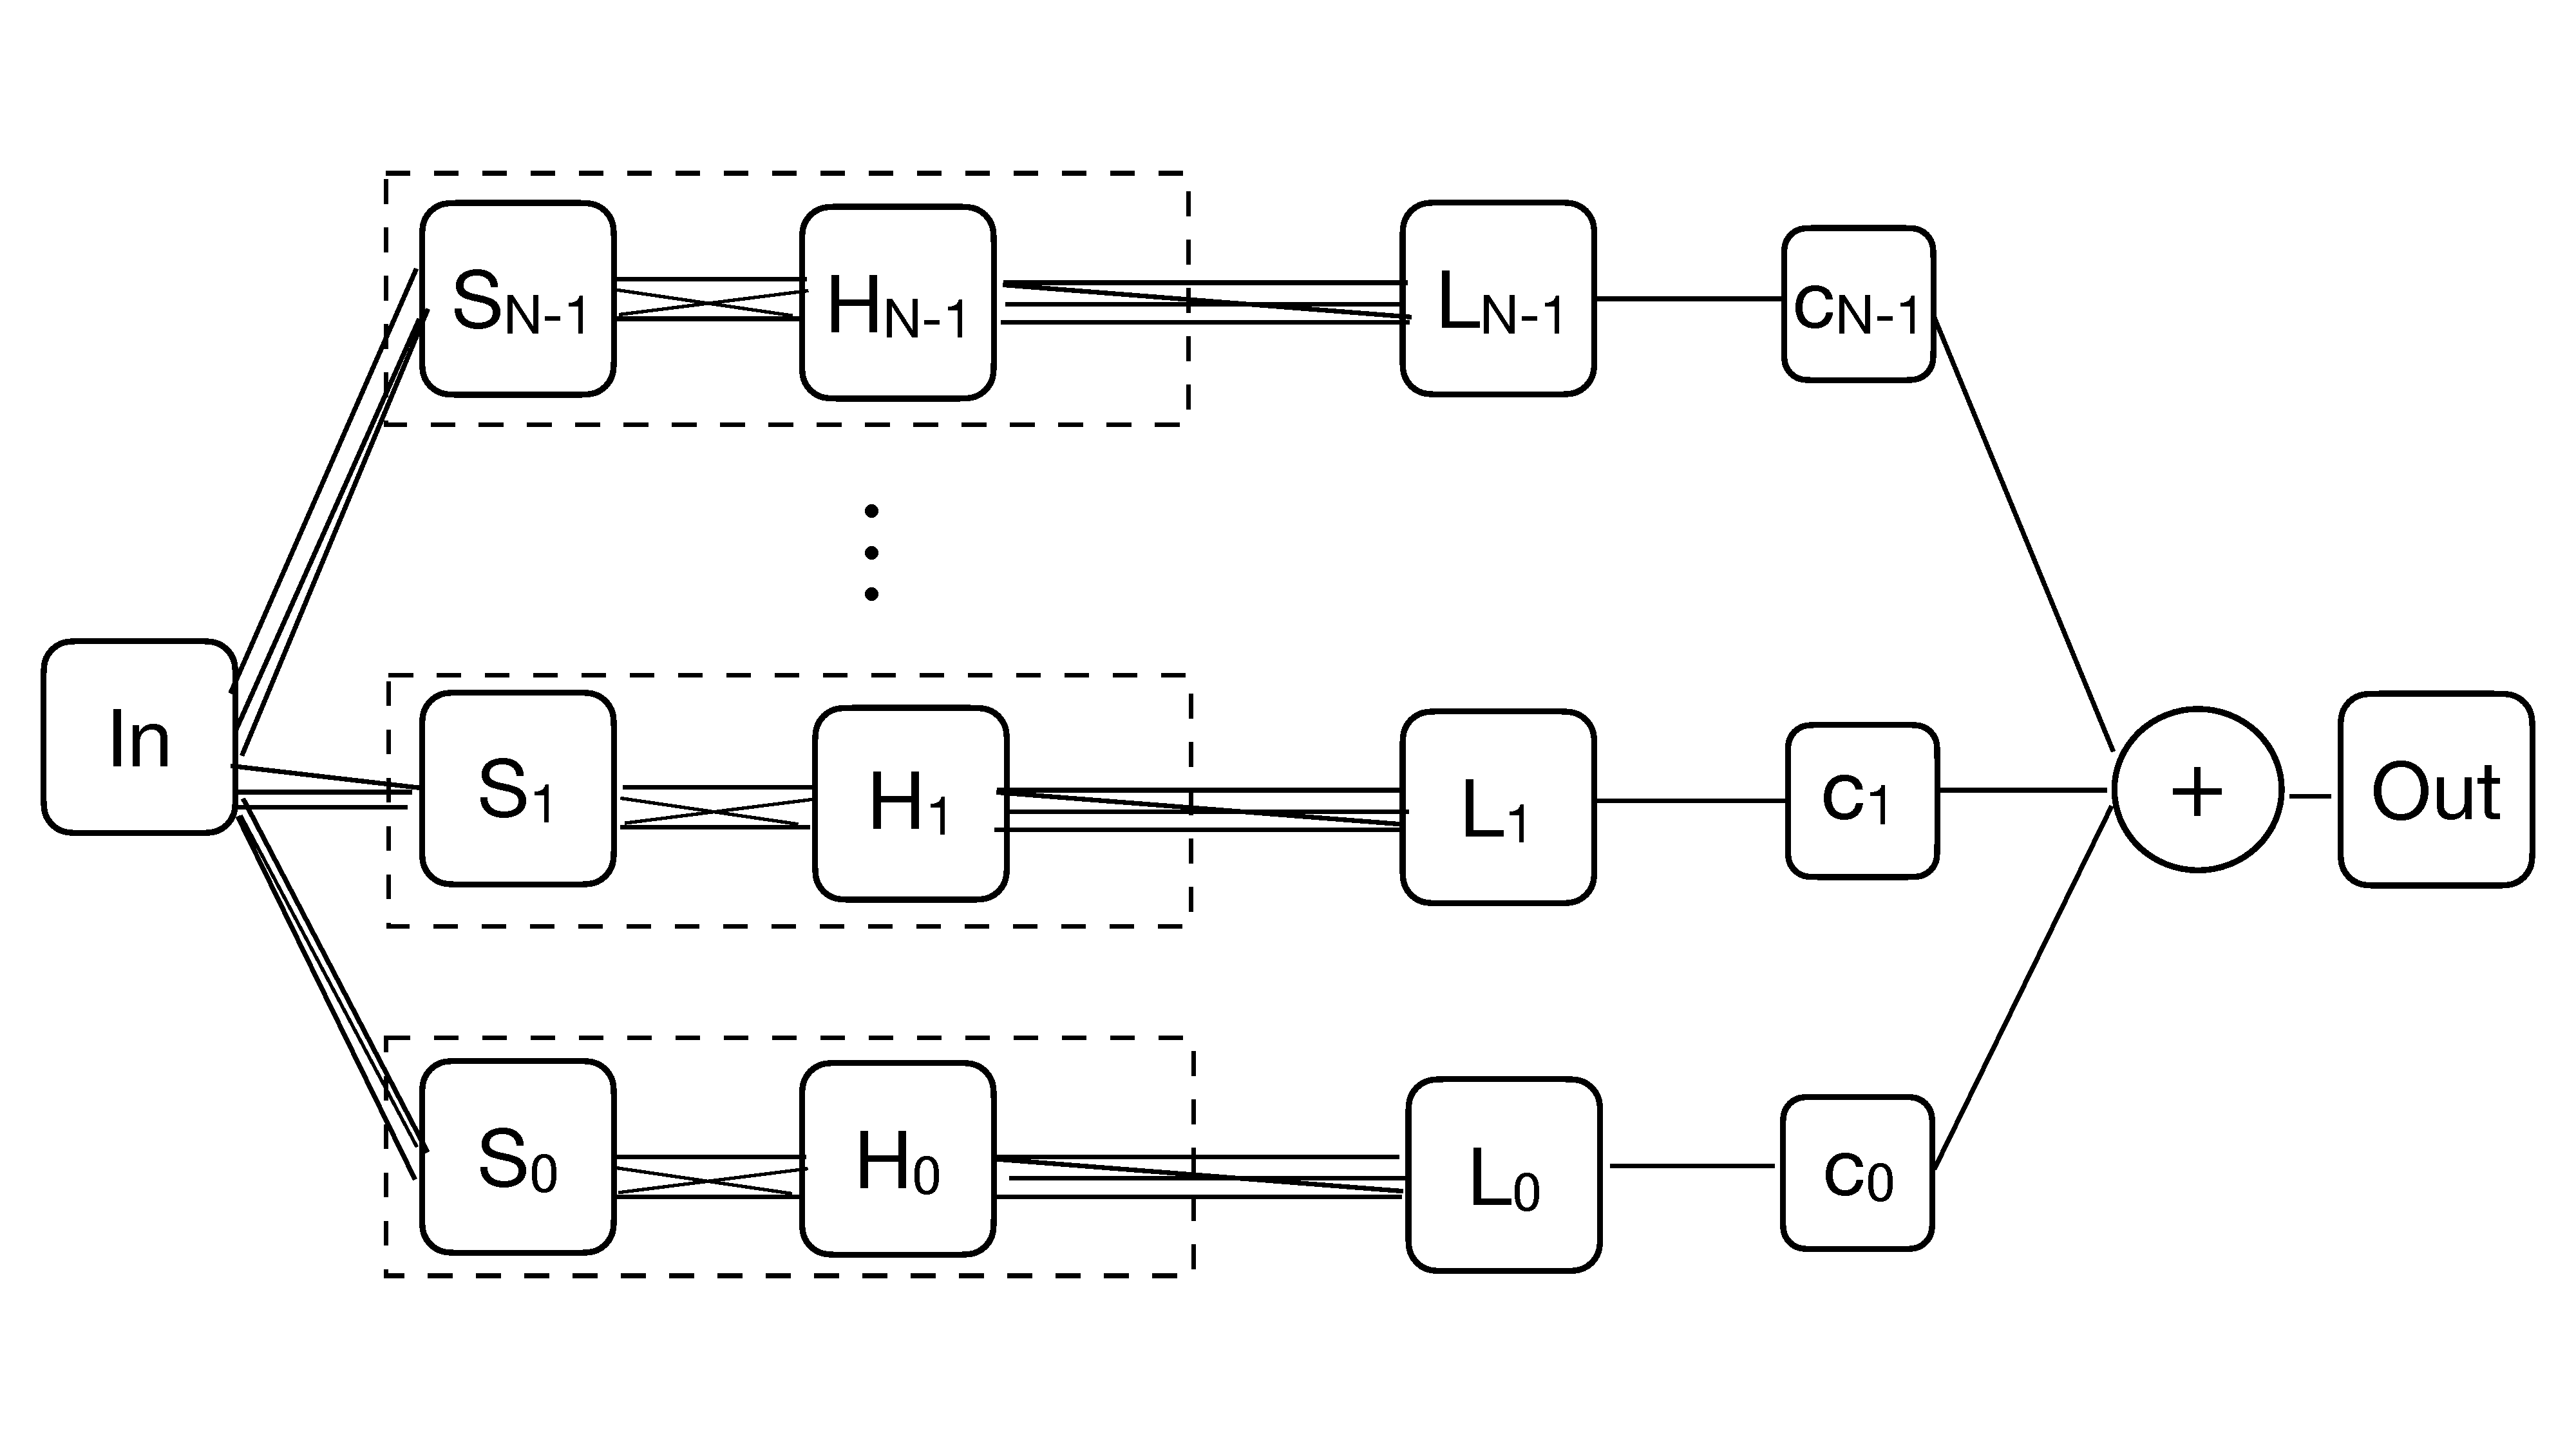
\includegraphics[width=0.7\linewidth]{img/ch4/lnet.pdf}
    \caption{L-Net architecture: Each stage is an independent modulated sine MR-Module, allowing for increased complexity and expressiveness.}
    \label{f:l-net}
\end{figure}

The key difference in the L-Net is the increased expressiveness due to the added depth of each stage. By incorporating the hidden block \( H_i \), each stage can model more complex compositions of sinusoidal functions, allowing the L-Net to capture finer details of the input signal quicker. As a result, the overall level of detail depends on the width and depth of the hidden block in each stage. 
% On the other hand, since the composition of sines generates much higher frequencies, it is not straightforward to bound the frequencies learned by the network.

An interesting property of the L-Net is that when considering the final stage at level \( N \), the function \( f(\cdot, N) \) \textit{behaves like a single deep sinusoidal} MLP. Without loss of generality, let \( f(x, t) = c_0(t)g_0(x) + c_1(t)g_1(x) \) be a two-stage L-Net with the same architecture for each stage, with a single hidden layer. Then, at \( t = 2 \), we show that the L-Net can be represented as \( f(x, 2) = L \circ H \circ S \), where \( L \), \( H \), and \( S \) combine the corresponding matrices of the stages. For this, define the matrices of $S$, $H$, and $L$, respectively, using $W_s\!=\!\begin{psmallmatrix}W_s^0\\W_s^1\end{psmallmatrix}$, 
$W_h\!=\!\begin{psmallmatrix}W_h^0& 0\\0&W_h^1\end{psmallmatrix}$, 
$W_l\!=\!\begin{psmallmatrix}W_l^0 & W_l^1\end{psmallmatrix}$, where $W_s^j$, $W_h^j$, $W_l^j$ are the matrices of the stages~$g_j$. The biases are defined similarly. This process generalizes to any \( N \)-stage L-Net in an analogous way, providing a controllable method to increase the effective \textit{width} of a sinusoidal MLP.

\subsection{M-Net: Hierarchical Modulated Stages}
\label{s-mnet}

Unlike the S-Net and L-Net, in which the stages are independent of each other, the M-Net introduces a hierarchical structure that reuses information learned at earlier stages. In the M-Net, each stage \( g_i \) is a modulated sine MR-Module that is \textit{directly linked to the subsequent stage} \( g_{i+1} \) through its hidden block as illustrated in Figure \ref{f:m-net}.

\begin{figure}[!h]
    \centering
    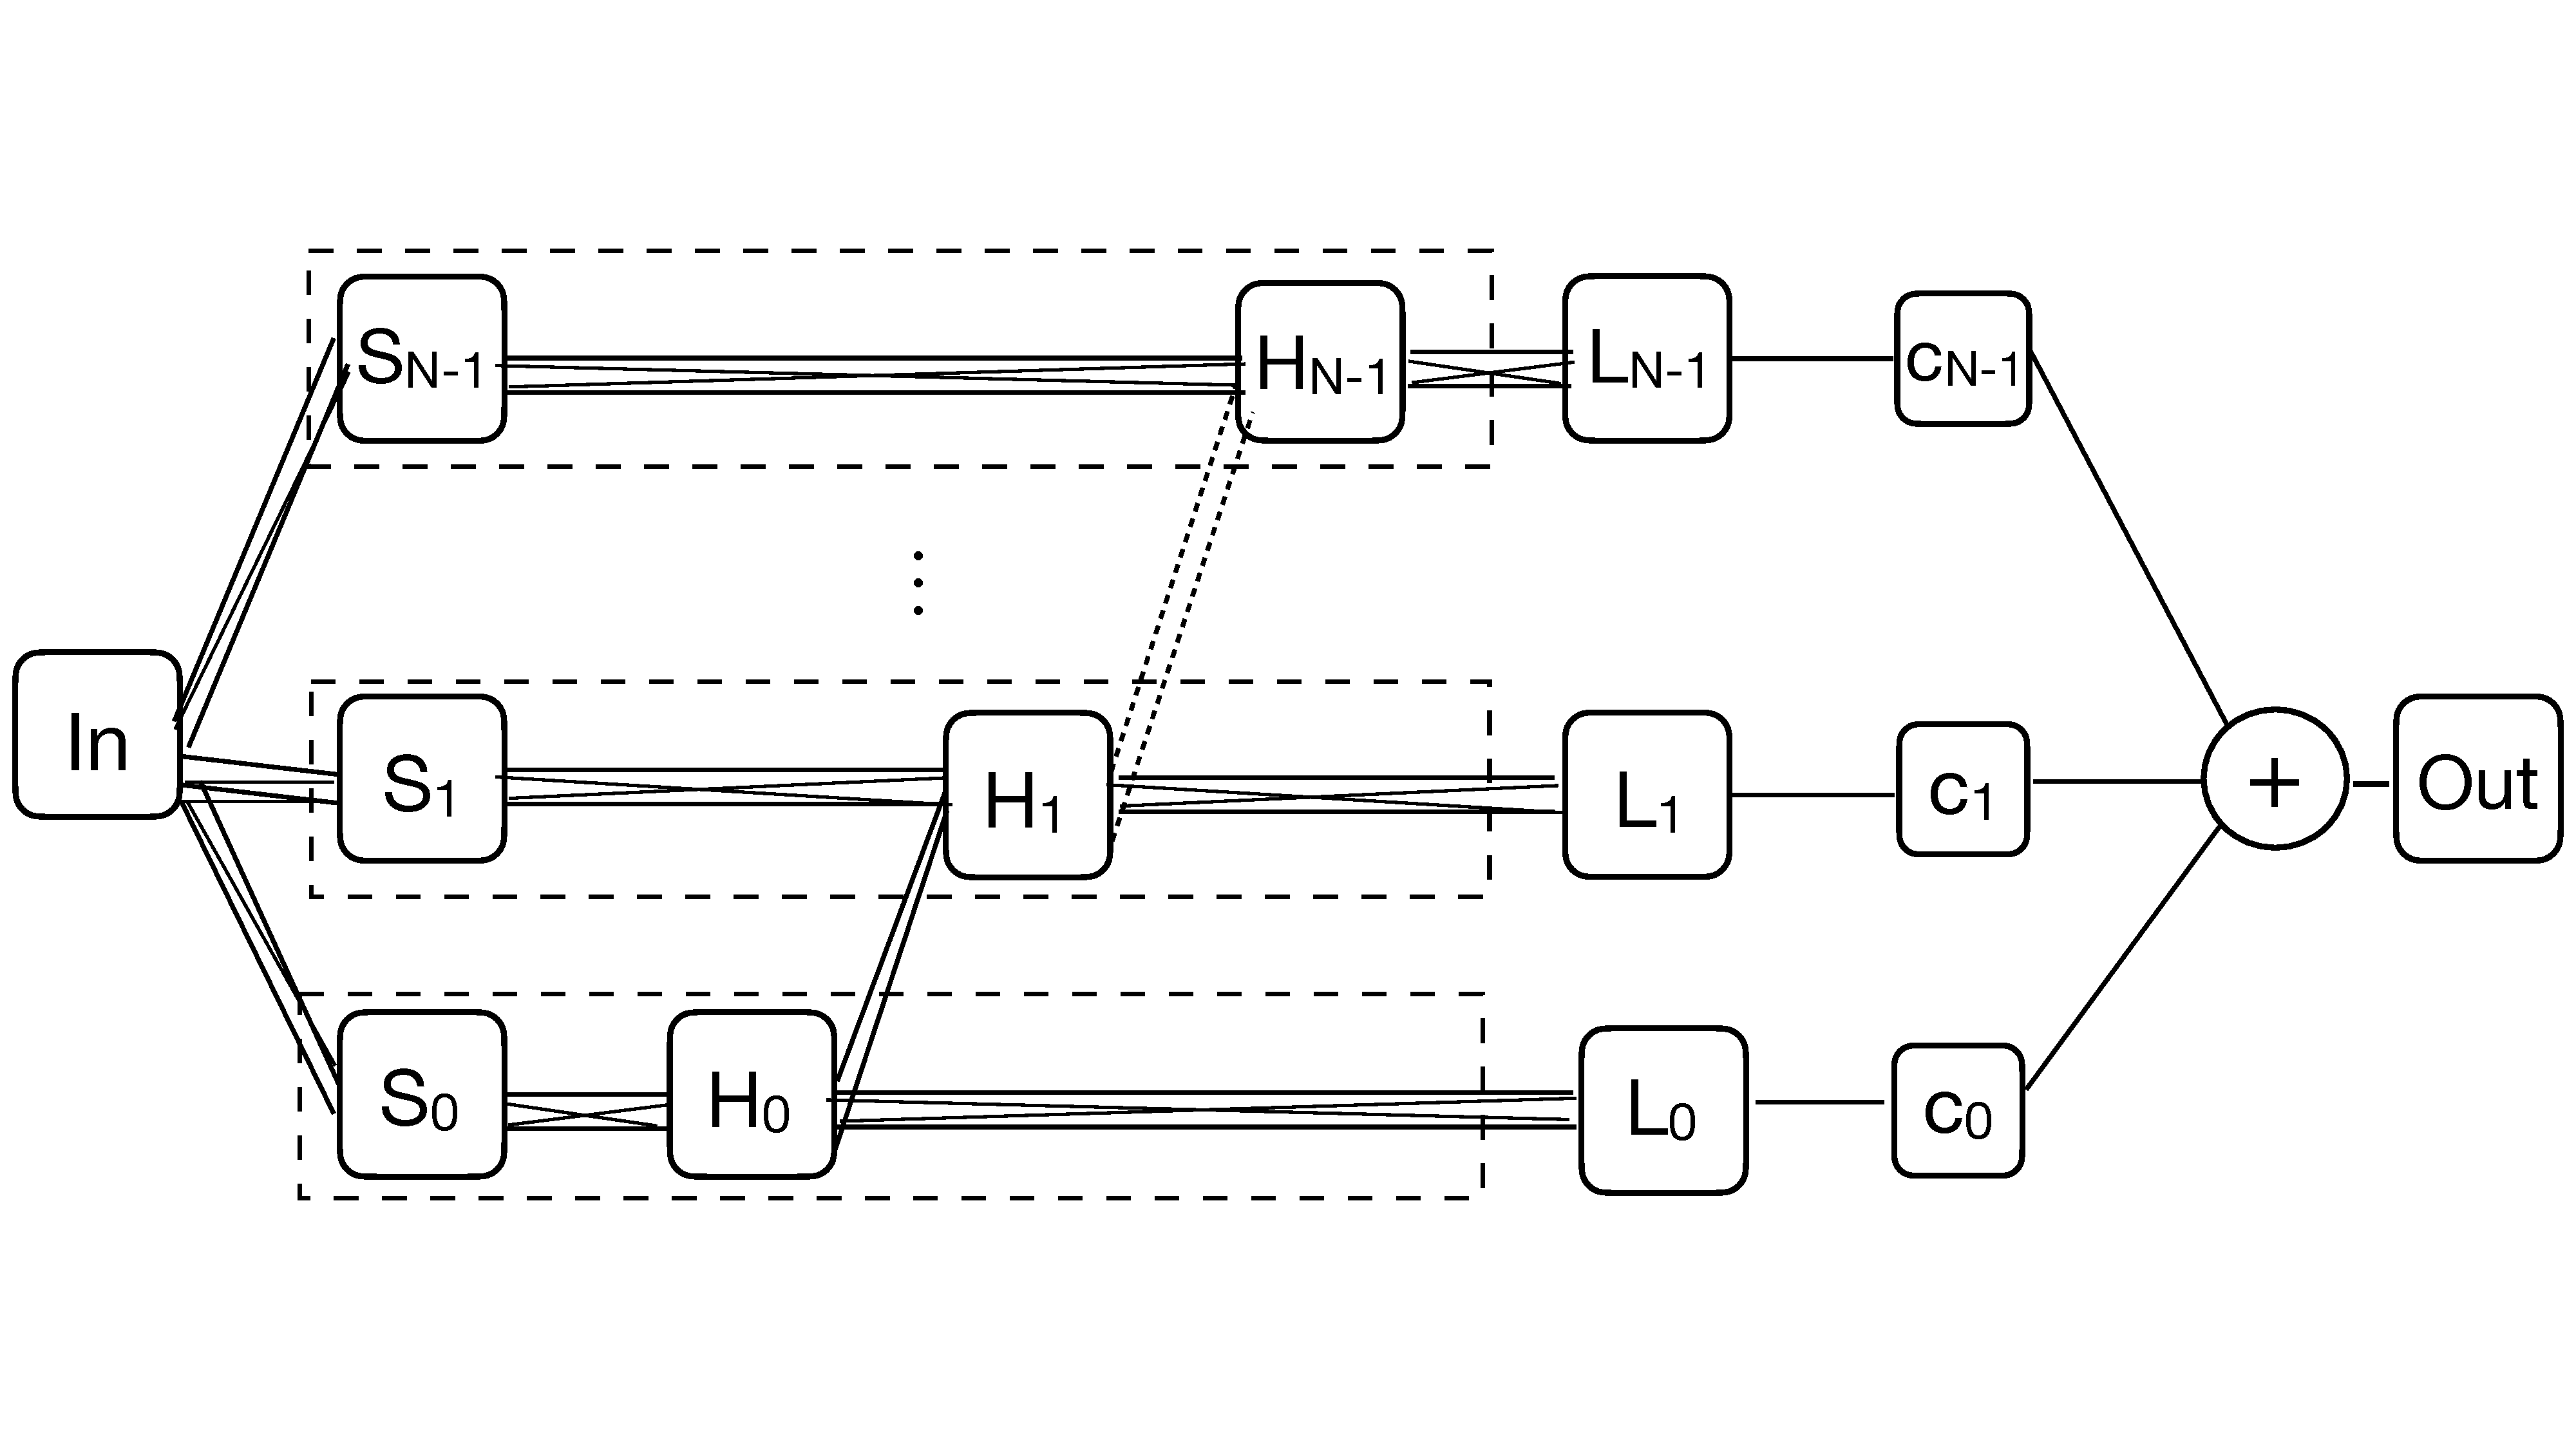
\includegraphics[width=0.75\linewidth]{img/ch4/mnet.pdf}
    \caption{M-Net architecture: Hierarchical connection between hidden layers allows for reuse of information and progressively refined representations.}
    \label{f:m-net}
\end{figure}
    
Specifically, $H_i\circ  S_i$ is composed both with the linear layer $L_i$, producing the stage $g_i\! =\! L_i\!\circ\! H_i\!\circ\!  S_i$, and the hidden block $H_{i+1}$ resulting in $g_{i+1}\! =\! L_{i+1}\!\circ H_{i+1}\!\circ\left(S_{i+1}, H_i\circ  S_i\right)$. This way, the the hidden block has the form $H_{i+1}\!:\!\R^{m_{i+1} + m_i}\!\to\! \R^{m_{i+1}}$; $m_i$ is the dimension of the output of the last hidden layer of stage $i$. 

This sequential linkage creates a hierarchical representation in which each stage can build upon and refine the features captured by previous stages. The overall M-Net can thus be viewed as a deep sinusoidal MLP with \( N \) hidden blocks:

\begin{align}
    f = L_{N-1} \circ \overline{H_{N-1}} \circ \cdots \circ \overline{H_1} \circ H_0 \circ S_0,
\end{align}

where \( \overline{H_i} \) represents the part of \( H_i \) that connects to stage \( g_{i+1} \).

This architecture provides a controllable way to increase the effective \textit{depth} of the sinusoidal MLP during training, making the M-Net particularly suitable for applications requiring compact multiresolution representations (see Section \ref{sec:considerations}).



\section{Multiresolution Training}\label{sec:mr_training}
\label{s:training}

The training of the MR-Net $f$ is inherently aligned with the hierarchical nature of its architecture, where each stage $g_i$ should contribute in representing a specific level of detail in the target signal $\gt{f}$. In a typical training strategy, MR-Net proceeds sequentially, starting with the lowest-frequency stage and gradually incorporating higher-frequency stages. This stage-wise learning approach allows the network to build a complete representation of the signal, beginning with coarse details and progressively refining the model with finer nuances. To ensure the integrity of the multiresolution representation, once a stage is trained to capture a particular level of detail, its weights are "frozen", preserving the learned coarse features as finer features are added incrementally.

The MR-Stages $\{g_i\}$ are the building blocks of the MR-Net $f$. They form a stack of MR-Modules that are interconnected according to the specific MR-Net subclass. The representation capacity of each stage $g_i$ can be fine-tuned by initializing its first layer to specific frequencies, adjusting the depth and width of the network, or incorporating ground-truth values $\gt{g}_i$ during training. The overall MR-Net configuration is defined by the parameters of its stages, including the number of stages, as well as the depth and width of each stage.


The MR-Net training process offers flexibility in terms of signal processing. Depending on the desired frequency characteristics for each stage, the input to MR-Net can either 
be the original ground-truth signal or a low-pass filtered version, supporting diverse multiresolution schemes.

In this section we describe each of the components in the training process in detail.

\red{As each stage is trained, it uses an adaptive loss functional that compares the network's output at that particular stage with the corresponding level of detail in the ground truth signal.}

% A key aspect of MR-Net training is the careful control of frequency representation at each stage. This control is achieved through specialized initialization techniques or by fine-tuning the width and depth of the network layers, ensuring that each stage captures its intended frequency band effectively.


% The capacity of $g_i$ to represent the underlying ground-truth stage $\gt{g}_i$ can be achieved by initializing its first layer, adjusting its width and depth, or by using the values $\gt{g}_i$ in training as explained in Section~\ref{s-frequency-control}. The input to the MR-Net during training can either be the original ground-truth signal or a pre-processed version using a low-pass filter, depending on the desired frequency characteristics for each stage.

% A key aspect of MR-Net training is the careful control of frequency representation at each stage. This is achieved through specialized initialization techniques or by fine-tuning the width and depth of the network layers. Such control ensures that each stage can effectively capture the appropriate frequency band of the signal.

% The training of the MR-Net $f$ must consider the mechanisms for learning different levels of detail at each stage $g_i$ of $f$. 

% Throughout the training process, a dedicated logger monitors progress, while a scheduler manages the progression through stages and epochs. This systematic approach to training allows the MR-Net to effectively capture and represent signals at various scales, providing a powerful framework for signal reconstruction and analysis.

% The MR-Training incorporates a \textit{loss functional}, a \textit{logger} to monitor the training, as well as, a \textit{scheduler} (see Fig~\ref{f:training}). We describe each of these components, as well as the multiresolution regime in the following sections. 

% \begin{figure}[!h]
% \centering
% 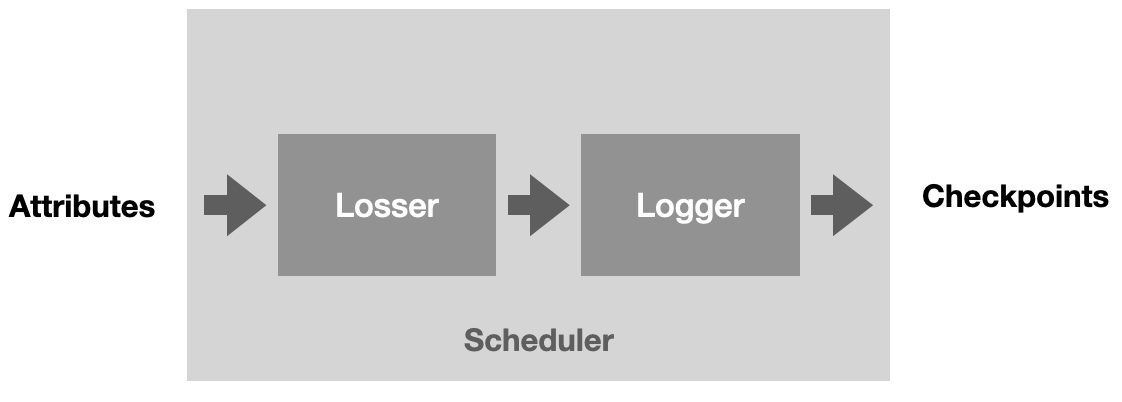
\includegraphics[width=0.89\linewidth]{img/ch4/training.png}
% \caption{MR-Training.}
% \label{f:training}
% \end{figure}

\subsection{Input Data}

% The training of MR-Net stage $g_i$ receives pairs $\{x_j, y_j\}$ as input, with points $x_j$ sampled in the domain $\mathcal{D}$ of $\gt{f}$ and $y_j=\gt{f}(x_j)\in~\mathcal{C}$, the contradomain. For instance, for a squared image, we could have $\mathcal{D}=[-1, 1]^2 \subset \R^{2}$. Note that, in general, spatial media objects like images or 3D models may be embedded in any region of their space. During training, we consider an image signal $\gt{f}$ to have codomain in a monochromatic ($\mathcal{C}=\R$) or trichromatic (eg. RGB) color space ($\mathcal{C}=\R^3$). Depending on the application, other color spaces or additional attributes, such as masks and features, could be used. We will explore other attributes in Chapter \ref{chap:seamless-textures}. Figure \ref{f:ex-signal-attributes} illustrate some of these attributes.

% The data input for the training of each of the $N$ stages $g_i$ is organized in a \textit{multi-stage stack} $\{x_j, y_j\}_i$. Specifically, for each $i$, the set of pairs $\{x_j, y_j\}_i$ is a sample of the $i$th level of detail $\gt{f}_i$ of the signal $\gt{f}$ or a sample of the original signal $\gt{f}$, with $\{x_j\}_i\subset \mathcal{D}$ and $\{y_j\}_i=\{\gt{f}_i(x_j)\}$. 
% From the point of view of \textit{representation theory}, we can interpret this as a projection of the function $\gt{f}_i$ onto the primal \textit{Shannon basis} (i.e., Dirac delta distribution). In the context of signal processing, this basis is a sampling grid of impulses and the representation consists of the sequence $\{y_j\}_i$ at the grid locations $\{x_j\}_i$.

% The type of sampling used to extract the multi-stage stack $\{x_j, y_j\}_i$ from the signal $\gt{f}$ is an important aspect in the MR-Net training. In that respect, it is instrumental to consider two types of samplings: \textit{regular} and \textit{irregular}. We will focus on the regular sampling, or uniform sampling, for which we have a well stablished and classic theory for sampling and reconstrcution. However, Chapter \ref{chap:future} briefly discusses some aspects that make irregular sampling interesting and could have more investigation.

Each MR-Net stage \( g_i \) is trained using pairs of samples \(\{x_j, y_j\}\), where \( x_j \) are points sampled from the domain \(\mathcal{D}\) of the ground-truth function \(\gt{f}\), and \( y_j = \gt{f}(x_j) \in \mathcal{C} \) are corresponding values in the codomain. For example, for a square image, the domain could be defined as \(\mathcal{D} = [-1, 1]^2 \subset \mathbb{R}^{2}\). Note that spatial media objects, such as images or 3D models, may be embedded in any region of their respective spaces. During training, an image signal \(\gt{f}\) can have codomains in a monochromatic space (\(\mathcal{C} = \mathbb{R}\)) or a trichromatic color space (\(\mathcal{C} = \mathbb{R}^3\)) as the RGB. Depending on the application, alternative color spaces or additional attributes, such as segmentation masks or feature maps, may also be used. We will explore these additional attributes in Chapter \ref{chap:seamless-textures}. Figure \ref{f:ex-signal-attributes} illustrates some possible attributes.

\begin{figure}[h]
    \centering
    \begin{subfigure}[b]{0.24\textwidth}
        \centering
        
\includegraphics[width=\textwidth]{img/placeholder512.png}
        \caption{RGB values}
    \end{subfigure}
    \begin{subfigure}[b]{0.24\textwidth}
        \centering
        
\includegraphics[width=\textwidth]{img/placeholder512.png}
        \caption{Monochromatic}
    \end{subfigure}
    \begin{subfigure}[b]{0.24\textwidth}
        \centering
        
\includegraphics[width=\textwidth]{img/placeholder512.png}
        \caption{Mask}
    \end{subfigure}
    \begin{subfigure}[b]{0.24\textwidth}
        \centering
        
\includegraphics[width=\textwidth]{img/placeholder512.png}
        \caption{Edges}
    \end{subfigure}
    \caption{Example of attributes and features that can be used in training}
    \label{f:ex-signal-attributes}
\end{figure}

For the training of each of the \( N \) stages \( g_i \), the input data is organized into a \textit{multi-stage stack} \(\{x_j, y_j\}_i\). Specifically, for each \( i \), the set of pairs \(\{x_j, y_j\}_i\) represents a sample from either the \( i \)-th level of detail \(\gt{f}_i\) of the signal \(\gt{f}\) or from the original signal \(\gt{f}\) itself, with \(\{x_j\}_i \subset \mathcal{D}\) and \(\{y_j\}_i = \{\gt{f}_i(x_j)\}\). The choice of sampling strategy to generate the multi-stage stack \(\{x_j, y_j\}_i\) from the signal \(\gt{f}\) is an important consideration in the MR-Net training.


\subsubsection{Sampling Strategies}

There are two primary sampling strategies: \textit{regular} and \textit{irregular} sampling. In this work, we focus on regular sampling, also known as uniform sampling, which is more commonly used and is supported by a well-established theoretical foundation for sampling and reconstruction. However, Chapter \ref{chap:future} briefly discusses some intriguing aspects of irregular sampling and highlights areas for future exploration.

In regular sampling, the points are arranged in a uniform grid \(\{x_{k,l}\}\) that discretizes the domain \(\mathcal{D}\). From the perspective of \textit{representation theory}, this setup can be interpreted as projecting the function \(\gt{f}_i\) onto the primal \textit{Shannon basis} (i.e., a grid of Dirac delta distributions). In the context of signal processing, this basis is a sampling grid of impulses, and the function is represented as the sequence \(\{y_j\}_i\) at the corresponding grid locations \(\{x_j\}_i\).

At the highest resolution, the points are structured in a square grid of size \( 2^k \) for some integer \( k > N \). The multi-stage grids \(\{x_{k,l}\}_i\) follow a dyadic lattice structure governed by the \( 2^i \) rule:

\begin{align}
    \{x_{k,l}\}_i = \{x_{2k, 2l}\}_{i+1}, \quad \text{where} \quad \{x_{k,l}\}_N = \{x_{k,l}\}.
\end{align}


This formulation ensures that each dimension of the grid \(\{x_{k,l}\}_i\) has twice the size of the previous stage grid, building a pyramid structure (see Figure~\ref{f:multi}(a)).

Alternatively, we can consider a fixed resolution for the sampling grids \(\{x_{k,l}\}_i\), where the signal \(\gt{f}\) is sampled at its highest level, or directly at the level of detail \(\gt{f}_i\) for each stage grid \(\{x_{k,l}\}_i\) (see Figure~\ref{f:multi}(b)). More details on this approach are provided in Section~\ref{s:lod}.


% Here we are assuming that $\{x_{k,l}\}$ is a grid of size $2^k\times 2^k$ for some integer $k>N$. Thus each dimension of a stage grid $\{x_{k,l}\}_i$ has twice the size of the previous one (Fig~\ref{f:multi}(a)). 
% On the other hand, we could consider that the sampling grids $\{x_{k,l}\}_i$ have a fixed resolution, and sample the signal $\gt{f}$ on its highest level or consider the level of detail $\gt{f}_i$ for each grid stage $\{x_{k,l}\}_i$ (Fig~\ref{f:multi}(b)). See Section~\ref{s:lod} for more details.

\begin{figure}[!h]
\centering
\begin{subfigure}{0.49\linewidth}
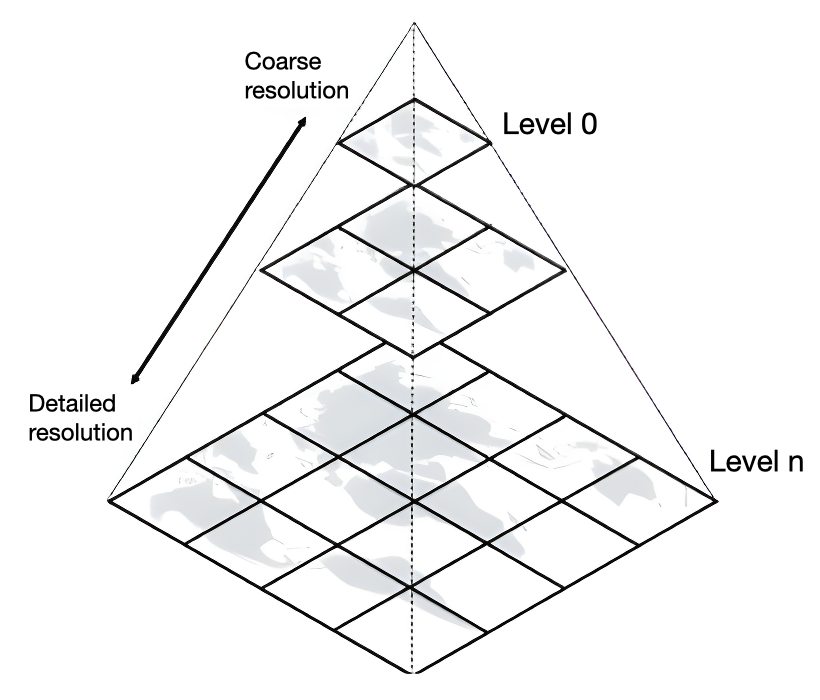
\includegraphics[width=\linewidth]{img/ch4/pyramid.png}
\caption{Pyramid Configuration}
\end{subfigure}
\begin{subfigure}{0.49\linewidth}
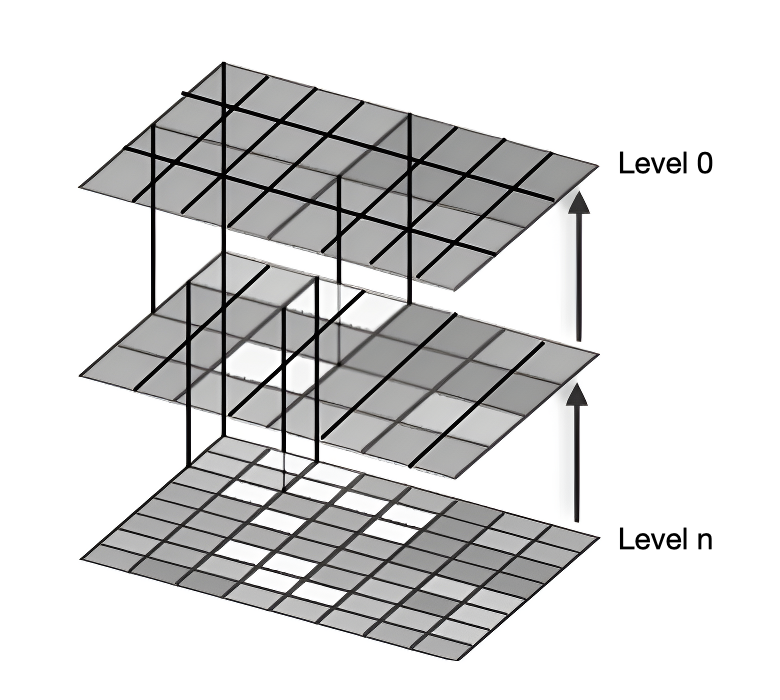
\includegraphics[width=\linewidth]{img/ch4/tower.png}    
\caption{Tower Configuration}
\end{subfigure}
\caption{Examples of multi-stage stack configurations.}
\label{f:multi}
\end{figure}

\subsubsection{Filtering Strategies}

Each level $i$ of the multi-stage stack can be filtered to separate the level of detail $\gt{f}_{i+1}$ into different frequency bands. In this context, we can use different variations of the signal \(\gt{f}\) for the stages, such as the unfiltered signal, a low-pass filtered version of \(\gt{f}_{i+1}\), or a band-pass filtered version of \(\gt{f}_{i+1}\). Usually, a Gaussian kernel is used for low-pass filtering, while a difference of Gaussians (DoG) kernel is used for band-pass filtering (see Figure~\ref{f:filter}).

The filtering operation is defined as follows: for a low-pass version of stage \(\gt{f}_{i+1}\), we convolve \(\gt{f}_{i+1}\) with a Gaussian kernel \( K \):
\begin{align}\label{e-gaussian-filter}
    \gt{f}_i(k,l) &= \left( K * \gt{f}_{i+1} \right)(k, l).
\end{align}

We abuse the notation slighly by denoting $\gt{f}_i(k,l)$ as the function $\gt{f}_i$ evaluated at the point $x_{k,l}$.
Similarly, the band-pass filtered stage \(\gt{g}_i\) is defined as the difference between the stage \(\gt{f}_i\) and its low-pass filtered version:
\begin{align}
    \gt{g}_i(k,l) = \left( \gt{f}_{i} - K * \gt{f}_{i} \right)(k, l).
\end{align}

% Each level \( i \) of the multi-stage stack can be filtered to isolate specific frequency bands, thereby refining the level of detail \(\gt{f}_{i+1}\) represented at that stage. In this sense, we can use the unfiltered signal $\gt{f}$, a low-pass version of $\gt{f}_{i+1}$ or a band-pass version of $\gt{f}_{i+1}$. For this, it is common to employ a Gaussian kernel as the low-pass kernel and a difference of Gaussians as the band-pass kernel (see Fig~\ref{f:filter}).

% Precisely, we can filter $\gt{f}_{i+1}$ by convolving it with a Gaussian kernel $K$:
% % and downsampling the result by a factor 2:
% \begin{align}\label{e-gaussian-filter}
%     \gt{f}_i(k,l)&=\left(K*\gt{f}_{i+1}\right)(k,l)
% \end{align}
% Here, we abuse the notation slightly by denoting \(\gt{f}_i(k,l)\) as the function \(\gt{f}_i\) evaluated at the point \( x_{k,l} \).

% Similarly, the $i$th band-pass stage $\gt{g}_i=\gt{f}_i-\gt{f}_{i-1}$ is defined using $\gt{g}_i(k,l)=\left(\gt{f}_{i}-K*\gt{f}_{i}\right)(k,l)$.

\begin{figure}[!h]
    \centering
    
\includegraphics[width=0.32\linewidth]{img/ch4/signal.png}
    
\includegraphics[width=0.32\linewidth]{img/ch4/gaussian.png}
    
\includegraphics[width=0.32\linewidth]{img/ch4/laplacian.png}\\
    {\hfil \hfil signal \hfil \hfil \hfil low-pass \hfil \hfil \hfil band-pass \hfil}
    \caption{Examples of filter types.}
    \label{f:filter}
\end{figure}


\pagebreak

\subsection{Level of Detail Schemes}
\label{s:lod}

By integrating the concepts introduced in the previous section, we can establish various strategies for learning level-of-detail representations using MR-Nets. The main schemes explored here are: Capacity-Based with Original Signal; Filtering with Gaussian/Laplacian Tower; and Filtering with Gaussian/Laplacian Pyramid.

\subsubsection{Capacity Based with Original Signal}
In this scheme, we train each stage $g_i$ of the MR-Net $f$ on the same sampling of the ground-truth signal $\gt{f}$, which is assumed to have no frequencies higher than a defined bandlimit $\omega$. The multi-stage stack $\{x_j, y_j\}_i$ used as input is composed of $N$ copies of the same sample $\{x_j, y_j\}$ of $\gt{f}$. As a result, \textit{every stage receives identical training data}, even if they vary in their ability to approximate the signal.

This approach leverages the fact that even when a sinusoidal neural network does not have enough capacity to perfectly reconstruct the ground-truth signal $\gt{f}$, it can still capture its lowest frequencies and reconstruct a smooth approximation of the signal when appropriately initialized, as discussed in Section~\ref{sec:capacity-filtering}. 


% \red{Figure \ref{f:capacity-filtering} illustrates this phenomenon by showing the reconstruction in 1D example. The MR-Net used in this case has a single stage with width $16$ and a single layer in all blocks.}
% \begin{figure}[!h]
% \centering
% 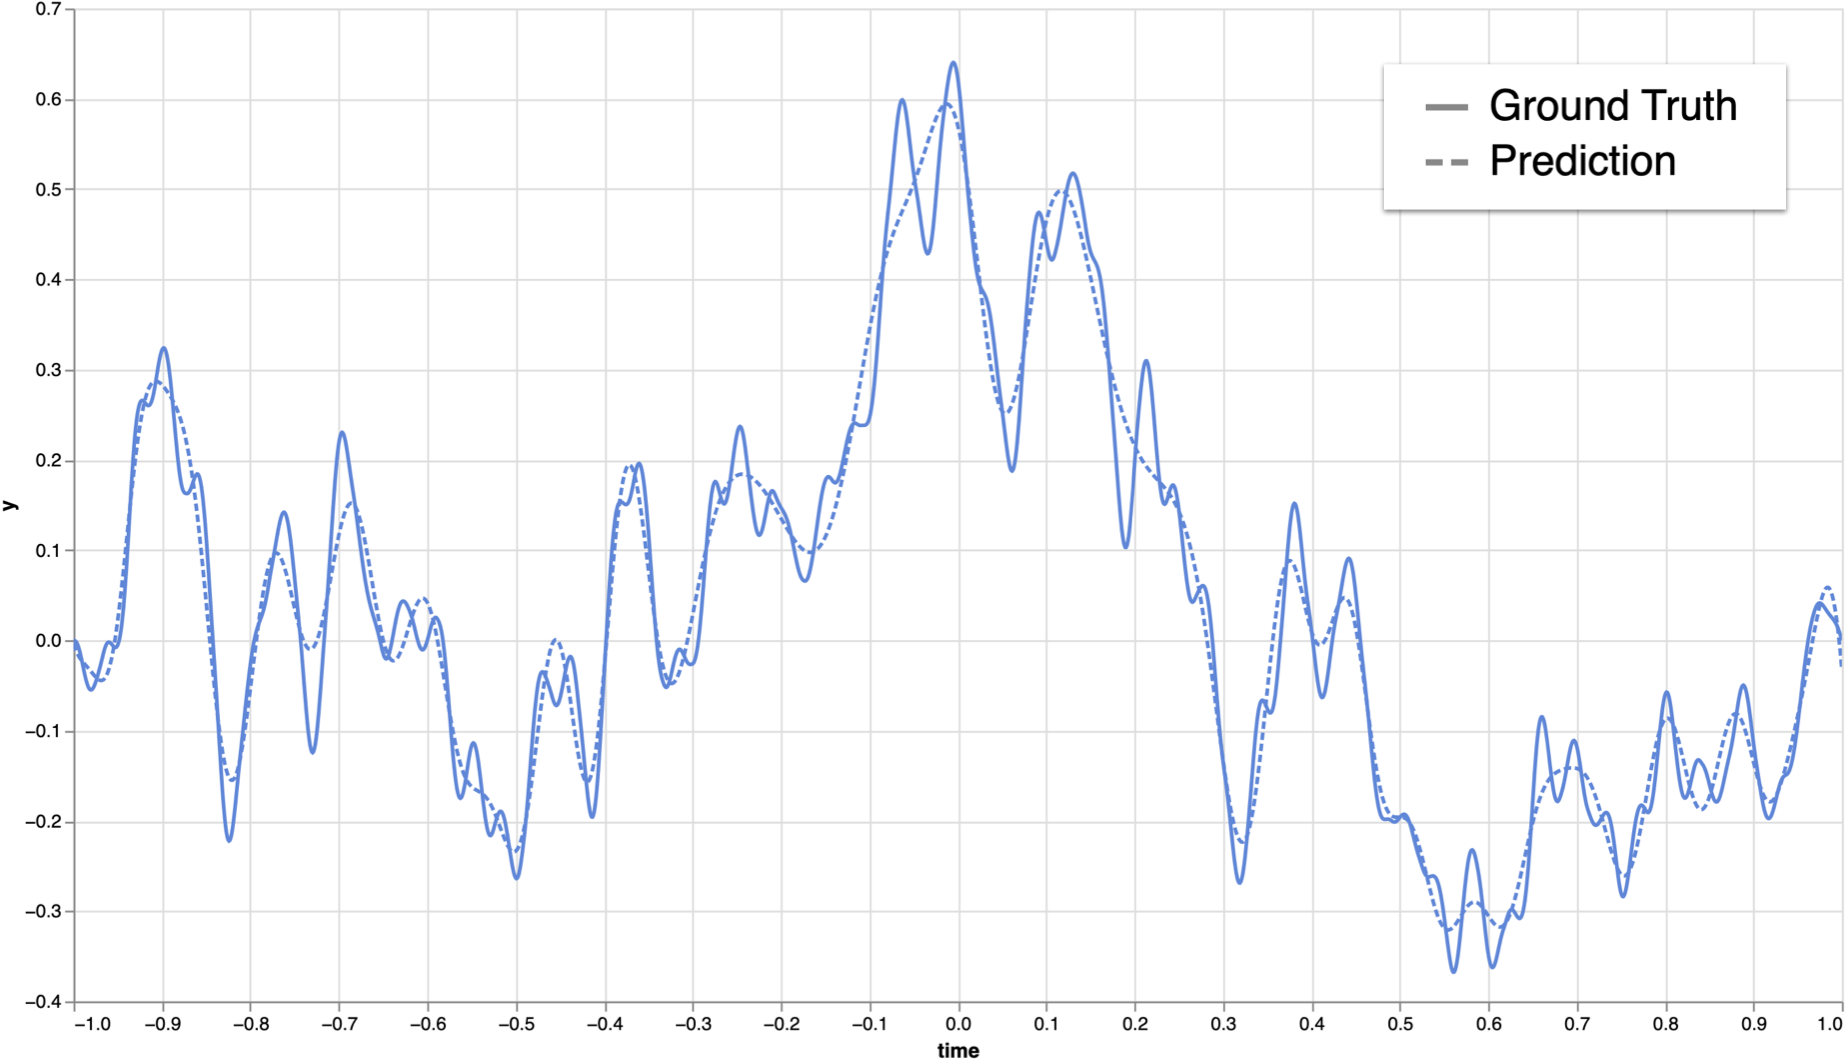
\includegraphics[width=\linewidth]{img/ch4/capacity-filtering.png}
% \caption{Illustration of capacity-based filtering in reconstructing a 1D signal.}
% \label{f:capacity-filtering}
% \end{figure}

The initialization of the $N$ stages $g_i$ of $f$ follows the scheme detailed in Section~\ref{s-frequency-initialization}. We set the rows of the first matrix of each stage $g_i$ with values in $\Omega_i=[-\omega_i, \omega_i]^2$, where $\omega_i$ is a partition of the interval $[0,\omega]$ and $\omega$ is the bandlimit of $\gt{f}$. Consequently, the first stage $g_0$ is configured to learn the lowest frequencies of $\gt{f}$ up to its capacity limit. As stages $g_1, g_2, \ldots, g_{N-1}$ are progressively added, each stage refines the learned representation, capturing additional levels of detail until the desired fidelity is achieved or the maximum number of stages is reached.


\subsubsection{Filtering with Gaussian / Laplacian Tower}

To achieve finer control over the frequencies present in the signal $\gt{f}$, we sample a filtered multi-stage stack $\{x_j, y_j\}_i$ and train each MR-Net stage $g_i$ to approximate the corresponding $i$ of this stack.

We start by constructing a *Gaussian tower*, a multi-stage stack $\{x_j, y_j\}_i$ where each level $i$ is derived by applying a low-pass filter to the preceding level $i+1$. Specifically, the Gaussian tower $\{x_j, y_j\}_i$ is generated recursively by convolving the \textit{level of detail} $\gt{f}_i$ of $\gt{f}$ with a Gaussian kernel $K$:
\begin{align*}
    \gt{f}_i(x_j) &= \left(K * \gt{f}_{i+1}\right)(x_j), \\
    \gt{f}_{N-1} &= \gt{f}.
\end{align*}

% Thus, we define $y_j=\gt{f}_i(x_j)$.
The attribute $y_j$ is defined as $\gt{f}_i(x_j)$. 
Each stage $g_i$ of the MR-Net is trained using the corresponding level $i$ of the Gaussian tower, from the less detailed scale to the most detailed one. Note that each level is trained using the same amount of samples. Moreover, we aim to minimize the loss $\mathcal{L}_i = \norm{f_i(x_j)-y_j}^2$, where $f_i = g_0 + \dots + g_{i}$.
% The MR-Net $f$ must be trained  using the loss $\mathcal{L}_i$ that minimizes the differences $\norm{f_i(x_j)-y_j}^2$, where $f_i=g_0+\dots+g_{i}$.

% Similarly, we could represent the multi-stage stack $\{x_j, y_j\}_i$ as a \textit{Laplacian tower} $\{\gt{g}_i\}$ by using:
% \begin{align*}
%     \gt{g}_i(x_j)&=\left(\gt{f}_{i}-K*\gt{f}_{i}\right)(x_j),\\
%     \gt{g}_0(x_j)&=\left(K*\gt{f}_{1}\right)(x_j).
% \end{align*}
% Thus, we define $y_j=\gt{g}_i(x_j)$ and train the MR-Net $f$ using the loss $\mathcal{L}_i$ that minimizes the differences $\norm{g_i(x_j)-y_j}^2$.

Alternatively, we can construct a \textit{Laplacian tower} $\{\gt{g}_i\}$ using:
\begin{align*}
    \gt{g}_i(x_j) &= \gt{f}_i(x_j) - \left(K * \gt{f}_i\right)(x_j), \\
    \gt{g}_0(x_j) &= \left(K * \gt{f}_1\right)(x_j).
\end{align*}
Here, $y_j = \gt{g}_i(x_j)$, and we train the MR-Net $f$ to minimize $\mathcal{L}_i = \norm{g_i(x_j)-y_j}^2$, where $g_i$ is the residual component at each stage.


\subsubsection{Filtering with Gaussian / Laplacian Pyramid}

Unlike the Gaussian tower, which is a highly redundant representation, the Gaussian pyramid is ``critically sampled,'' i.e., it uses the minimum number of samples necessary to represent each frequency band.

The Gaussian pyramid $\{x_{k,l}, y_{k,l}\}_i$ is defined by recursively downsampling each level of the Gaussian tower of $\gt{f}$ by a factor of 2. We assume the sampled points $\{x_{k,l}\}$ form a grid of size $2^k$ for some integer $k>N$. Thus, each dimension of a stage grid $\{x_{k,l}\}_i$ is half the size of the previous level's grid.

Similarly, the \textit{Laplacian pyramid} is built using the Laplacian tower of $\gt{f}$, applying downsampling to the residual components.

From the experiments in Section \ref{sec:generalization}, we conclude we can generalize correctly the model based only on the samples of a Gaussian pyramid. In terms of efficiency, it's faster to train the model on fewer samples, aligned with classical sampling theory results. This way, the Gaussian pyramid representation is more efficient and compact than the Gaussian tower. 

When training with a multi-stage stack with grids of different resolutions such as a Gaussian pyramid, we can build another multi-stage stack where each level has the same resolution as the original signal and use it as test data. In this case, this second multi-stage stack, a tower, should have each level filtered accordingly to its corresponding level in the pyramid, so that they are separated in similar frequency bands. With this pre-processing, we can train the network on the multiresolution pyramid data, and evaluate it on the original signal resolution, comparing it against the multiresolution tower data to check if the model is generalizing as expected.

When training with a Gaussian/Laplacian pyramid, we initialize the stages $g_i$ of $f$ based on a dyadic sequence of frequency bands:
\[
\omega_{N-1}, \frac{\omega_{N-1}}{2}, \ldots, \frac{\omega_{N-1}}{2^{N-1}},
\]
where $\omega_{N-1} = 2^{k-1}$. Each stage $g_i$ is initialized using the set $\Omega_i = \left[-\omega_i, \omega_i\right]^2$ for the first layer of $g_i$, ensuring that the frequency ranges align with the pyramid structure and maintain the desired resolution properties.

% The \textit{Gaussian pyramid} is a classical multiscale representation of uniformly sampled signals. Based on the Shannon sampling theorem, the Gaussian tower is a highly redundant multiscale representation. On the other hand, the Gaussian pyramid is ``critically sampled'', i.e., it has the minimum number of samples required to represent each frequency band. 

% As in Section~\ref{sec:mr_struct}, we are assuming that the sampled points $\{x_{k,l}\}$ forms a grid of size $2^k\times 2^k$ for some integer $k>N$.
% Thus each dimension of a stage grid $\{x_{k,l}\}_i$ has twice the size of the previous one

% As shown in Section~\ref{sec:generalization}, a model can generalize correctly when trained on the Gaussian pyramid's fewer samples, 
% making it ideal for tasks requiring a reduced dataset size while retaining frequency information. 

% To evaluate performance on the original signal, we can generate a multi-stage stack where each level has the same resolution as $\gt{f}$ and use it as the test data. This test stack, known as a Gaussian/Laplacian tower, is obtained by applying the corresponding filtering operations to each level of the pyramid. By training on the multi-resolution pyramid and testing on the reconstructed tower, we can validate whether the MR-Net is correctly generalizing to the full-resolution signal.


% The training of the MR-Net stages $g_i$ using Gaussian/Laplacian is analogous to the tower's case.
% Regarding the initialization of $g_i$, observe that $2^{k-N+1+i}$ is the height and width of the $i$th stack $\{x_{k,l}, y_{k,l}\}_i$, thus it cannot contain frequencies higher than $\omega_i=2^{k-N+i}$. 
% Thus we propose to initialize the frequencies of $\{g_i\}$ following a dyadic sequence of frequency bands 
% $\omega_{N-1}, \omega_{N-2}, \ldots, \omega_{0},$
% which is equivalent to $$\omega_{N-1}, \frac{\omega_{N-1}}{2}, \ldots, \frac{\omega_{N-1}}{2^{N-1}} \text{ with } \omega_{N-1}= 2^{k-1}.$$
% These are the bandlimits used to define the sets $\Omega_i=\left[-\omega_i, \omega_i\right]^2$ to initialize the frequencies of the first layer of each stage $g_i$.


% In practice, we assume that the data is given as a regular sample (digital image) of size $2^{k}\times 2^k$
% of the ground-truth signal~$\gt{f}$.
% We abuse the notation by denoting this digital image by~$\gt{f}$.
% To train the MR-Net stages~$\{g_i\}$, we use the (discrete) \textit{Gaussian} and \textit{Laplacian} pyramids of $\gt{f}$, both with $N<k$ levels.
% Precisely, the Gaussian pyramid $\{\gt{f}_i\}$ is defined recursively by convolving the \textit{level of detail} $\gt{f}_i$ with a Gaussian kernel $K$ and downsampling the result by a factor 2:
% \begin{align*}
%     \gt{f}_i(k,l)&=\left(K*\gt{f}_{i+1}\right)(2k,2l)\,\, \text{with} \,\, k,l\in \left\{1,\ldots, 2^{k-N+1+i}\right\},\\
%     \gt{f}_{N-1}&=\gt{f}.
% \end{align*}
% $\gt{f}_i(k,l)$ denotes the digital image $\gt{f}_i$ evaluated at the pixel $(k,l)$.
% Similarly, the Laplacian pyramid $\{\gt{g}_i\}$ is defined using
% \begin{align*}
%     \gt{g}_i(k,l)&=\left(\gt{f}_{i}-K*\gt{f}_{i}\right)(2k,2l)\,\, \text{with} \,\, k,l\in \left\{1,\ldots, 2^{k-N+1+i}\right\}\\ \gt{g}_0(k,l)&=\left(K*\gt{f}_{1}\right)(2k,2l).
% \end{align*}

\subsection{Frequency Control and Initialization}
\label{s-frequency-initialization}


Let $\gt{f}=\gt{g}_0+\cdots+\gt{g}_{N-1}$ be the ground-truth signal in multiresolution, and $f:\R^d\times [0,N]\to \R^n$ be a MR-Net with $N$ stages. To train each stage $g_i$, we propose to initiate its parameters based on the frequency content of $\gt{g}_i$.
There are two ways to control the frequency band of $g_i$. First, we can initialize the weight matrix of the first layer of $g_i$. Second, we can vary its width and depth. Moreover, these mechanisms can be combined.

Regarding the initialization of the MR-Net $f$, let $g_i=L_i\circ H_i\circ S_i$ be its $i$th stage, where $S_i$, $H_i$, and $L_i$ are its first, hidden, and linear blocks.
Observe that each coordinate of the sinusoidal layer $S_i(x)=\sin\left(W_{s_i} x+b_{s_i}\right)$ has the form $\sin(\omega_1 x_1 +\omega_2 x_2 + \varphi)$, where the \textit{frequencies} $\omega_1$ and $\omega_2$ form a line of the matrix $W_{s_i}$, $x=(x_1,x_2)$ is the input, and the \textit{phase-shift} $ \varphi$ is a coordinate of the bias $b_{s_i}$. 

Following the experiments and conclusion presented in Chapter \ref{chap:sinusoidal}, we initialize the first sinusoidal layer of each stage using a value of $\omega_0$ that determines a \textit{bandlimit frequency} related to the ground-truth stage $\gt{g}_i$. The weights of the hidden block $H_i$ are initialized following the same scheme in \cite{sitzmann2019siren}.

Ideally, the initialization of frequencies in $g_i$ should match the frequency content of the ground-truth signal at the stage $\gt{g}_i$. However, as we usually don't have access to this information, we opt to use an upper bound. Specifically, we assume that $\gt{g}_i$ has no frequency higher than a \textit{bandlimit} $B_i$. The Nyquist–Shannon sampling theorem says that we can reconstruct $\gt{g}_i$ from a sample $\{\gt{g}_i(x_{kl})\}$, where the regular grid $x_{kl}$ has points spaced with size $\frac{1}{r_i}<\frac{1}{2B_i}$. The number $r_i$ is the \textit{sample rate}. Figure \ref{f:nyquist} illustrates such requirement using the frequency rate notation.  

\begin{figure}[!h]
\centering
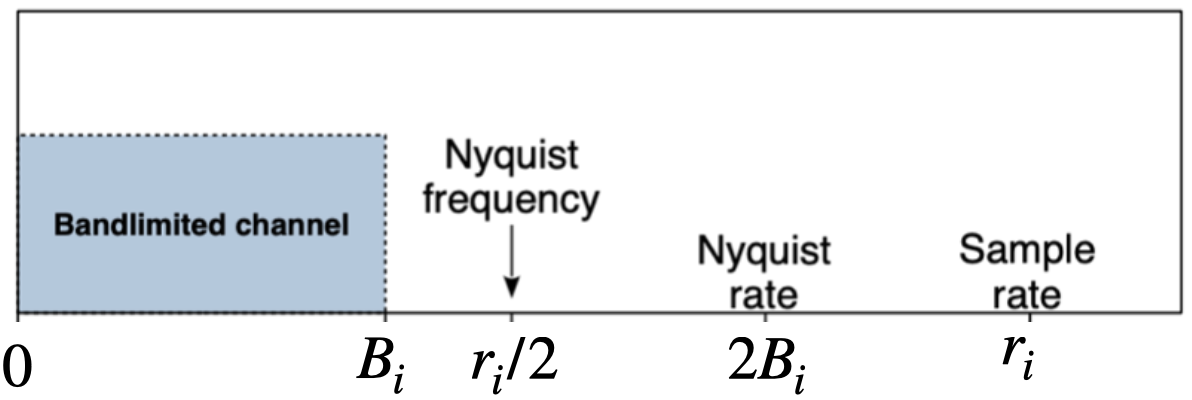
\includegraphics[width=0.7\linewidth]{img/ch4/nyquist.png}
\caption{Nyquist Limit.}
\label{f:nyquist}
\end{figure}


Therefore, to fit the stage $g_i$ to the sample $\{\gt{g}_i(x_{kl})\}$, we opt to initialize $g_i$ such that it can represent frequencies up to $\omega_i:=\frac{r_i}{2}$.
\red{For this, we initialize the lines of the first matrix $W_{s_i}$ of $g_i$ uniformly in the set $\Omega_i=\left[-\omega_i, \omega_i\right]^2$. DIVIDIR POR 16 SEPARAR S-NET das demais} 
Thus, the sinusoidal layer $S_i$ may contain frequencies already initialized at previous stages because $\{\gt{g}_i\}$ is a Laplacian pyramid of $\gt{f}$, thus, $\Omega_0\subset \cdots \subset \Omega_{N-1}$. 

\subsection{Loss Functional}

Signal reconstruction is related to interpolation and fitting. We would like to fit the MR-Net $f$ to the ground-truth signal $\gt{f}$ using a given sample of $\gt{f}$.
For this, we observe that training $f$ is related to a \textit{regression} in multi-scale. This means that: i) the approximation should take into account a multiresolution $\gt{f}=\gt{g}_0+\cdots+\gt{g}_{N-1}$ of the ground-truth signal; and ii) each MR-Net stage $g_i$ should fit to a sample of $\gt{g}_i$.

To accomplish these goals above, we define a \emph{loss functional} $\mathcal{L}_i$ to train each stage $g_i$ of the MR-Net $f$. For this, we assume that the signal $\gt{f}$ was sampled and organized in a \textit{multi-stage stack} $\{x_j, y_j\}_i$ such that $y_j=\gt{g}_i(x_j)$. Thus $\mathcal{L}_i$ is defined by minimizing the differences between the true values $y_j$ at the sample points $x_j$ and the predicted values $g(x_j)$ at the $i$th stage: 

\begin{align}\label{e-loss}
    \mathcal{L}_i(\theta_i)=\frac{1}{K_i}\sum \norm{g_i(x_j)-y_j}^2.
\end{align}

Where $\theta_i$ are the parameters of $g_i$ and $K_i$ is the size of $\{x_j, y_j\}_i$.

When the multi-stage stack $\{x_j, y_j\}_i$ is constructed by filtering $\gt{f}$ using a Gaussian filter (Eq~\ref{e-gaussian-filter}), we should replace $\norm{g_i(x_j)-y_j}$ by $\norm{f_i(x_j)-y_j}$ in Eq~\ref{e-loss}, recall that $f_i$ is the $i$th level of detail of the MR-Net $f$, i.e. $f_i=g_0+\dots+g_{i}$.

% Consequently, a good loss function bridges the gap between the data and the functional model.
% The most common \textit{norms} for regression problems use the $L^1$ and $L^2$ norms.

% During training, the network can be over-fitted to the data. To avoid this, we explore regularization strategies such as defining convergence criteria for early stopping to fit the network to the data. In the future, we plan to enhance these strategies by adding \textit{regularization terms} based on network derivatives. 


% Notice that we are working with representational neural networks, that is, a neural network that is trained to represent a single signal. This way, the over-fitting and generalization problem.

\subsection{Scheduler}

% Since a MR-Net $f$ has $N$ stages $g_i$, each learning a level of detail of the ground-truth signal $\gt{f}$, one important aspect is their training schedule. 
The multiresolution training is governed by a training scheduler that organizes the training sequence and apply regularization strategies based on convergence criteria. In general, it may be beneficial to train each stage sequentially, from the lowest to the highest level. This scheduling is our choice for our experiments and a common strategy in the traditional multiresolution analysis of signals. However, if the input multi-stage stack $\{x_j, y_j\}_i$ is organized as a Laplacian pyramid and $f$ is a L-Net, it is possible to train all stages in parallel by summing the loss functions $\mathcal{L}_i$ of the MR-stages. 

Furthermore, we adopt a progressive learning strategy by "freezing” the weights of a stage once it is trained in the scheduled sequence. This strategy guarantees that the details are added to the representation incrementally from coarse to fine.

We also employ an adaptive training scheme for each stage optimization combining both accuracy loss thresholds and convergence rates. The training process is outlined in Algorithm~\ref{alg:mr-training}.

\begin{algorithm}[hbt!]
\caption{MR-Net training.} \label{alg:mr-training}
\KwData{A multi-stage stack $\{x_j, y_j\}_i$ with $N$ levels.}
\KwResult{A MR-Net $f$ with $N$ stages $g_i$.}
    Initialize a MR-Net model with a single stage $g_0$\;
    Notify Logger that network training will start\;
    \For{$stage\gets0$ \KwTo $N-1$}{
        \If{$stage\neq~0$}
        {
            Create a new stage $g_{stage}$ and add it to the model\;
            Freeze the parameters of the stage $g_{stage-1}$\;
        }
        Notify Logger that stage training will start\;
        $\texttt{current\_traindata}~\!\!\gets~\!\!\texttt{multires\_stack}[stage]$\;
        \For{\normalfont $epoch\gets 0$ \KwTo \texttt{current\_limit\_of\_epochs}}{
            \For{\normalfont \textit{batch} in \texttt{current\_traindata}}{
                Train $g_{stage}$ using the loss $\mathcal{L}_{stage}$ (Eq~\ref{e-loss}) \;
                Notify Logger that batch training has finished\;
            }
            Notify Logger that epoch training has finished\;
            \If{\normalfont\texttt{convergence\_criteria\_reached()}}
                {\textbf{break}\;}
        }
        Notify Logger that stage training has finished\;
    }
    Notify Logger that network training has finished\;
\end{algorithm}

\pagebreak

\section{Multiresolution Inference}

Arguably, the primordial purpose of a signal representation is to provide an accurate reconstruction of the underlying data. Moreover, in the ideal case, the reconstruction method should be able to work with a continuous model of the signal, generating signal values at arbitrary points of its domain.

In that respect, coordinate-based neural networks features a compact model of the signal as a continuous function. Additionally, our MR-Net architecture gives a representation that is continuous both at space and scale. 
Therefore, it can reconstruct the signal zooming in and out at any desired level of detail by specifying a value $t$ to adjust the control layer coefficients, during the inference, according to Equations \ref{e-mrnet} and \ref{e-control}.

These characteristics are very important in media applications. In particular, there is a need to control the signal reconstruction for rendering, thus making it adapted to display resolution. The MR-Net architecture subsumes a model that incorporates filtering of the signal's frequency content in a controlled manner. This capability is crucial for \textbf{antialiasing} treatment, necessary to avoid visual artifacts when rendering the signal.

The MR-Net representation as a hierarchy of levels of detail has implications for transmission and processing of the signal. On one hand, regarding the former, it is possible to send coarse versions of the signal, quickly through a channel and subsequently update the level of detail for progressive renderings. On the other hand, concerning the latter, level of detail facilitates data caching using the different memory structures of the GPU.

% \section{MR-Framework}


% % \vspace{0.2cm}
% % {\color{red}
% % In practice, we assume that the data is given as a regular sample (digital image) of size $2^{k}\times 2^k$
% % of the ground-truth signal~$\gt{f}$.
% % We abuse the notation by denoting this digital image by~$\gt{f}$.
% % To train the MR-Net stages~$\{g_i\}$, we use the (discrete) \textit{Gaussian} and \textit{Laplacian} pyramids of $\gt{f}$, both with $N<k$ levels.
% % Precisely, the Gaussian pyramid $\{\gt{f}_i\}$ is defined recursively by convolving the \textit{level of detail} $\gt{f}_i$ with a Gaussian kernel $K$ and downsampling the result by a factor 2:
% % \begin{align*}
% %     \gt{f}_i(k,l)&=\left(K*\gt{f}_{i+1}\right)(2k,2l)\,\, \text{with} \,\, k,l\in \left\{1,\ldots, 2^{k-N+1+i}\right\},\\
% %     \gt{f}_{N-1}&=\gt{f}.
% % \end{align*}
% % $\gt{f}_i(k,l)$ denotes the digital image $\gt{f}_i$ evaluated at the pixel $(k,l)$.
% % Similarly, the Laplacian pyramid $\{\gt{g}_i\}$ is defined using
% % \begin{align*}
% %     \gt{g}_i(k,l)&=\left(\gt{f}_{i}-K*\gt{f}_{i}\right)(2k,2l)\,\, \text{with} \,\, k,l\in \left\{1,\ldots, 2^{k-N+1+i}\right\}\\ \gt{g}_0(k,l)&=\left(K*\gt{f}_{1}\right)(2k,2l).
% % \end{align*}
% % Since $2^{k-N+1+i}$ is the height and width of $\gt{g}_i$, it cannot contain frequencies higher than $\omega_i=2^{k-N+i}$. 
% % Thus we propose to initialize the frequencies of the $N$ stages $\{g_i\}$ of the MR-Net $f$ following a dyadic sequence of frequency bands 
% % \begin{align}
% % \omega_{N-1}, \omega_{N-2}, \ldots, \omega_{0}.
% % \end{align}
% % Which is equivalent to $\omega_{N-1}, \frac{\omega_{N-1}}{2}, \ldots, \frac{\omega_{N-1}}{2^{N-1}}$ with $\omega_{N-1}= 2^{k-1}$.
% % These are the bandlimits used to define the sets $\Omega_i=\left[-\omega_i, \omega_i\right]^2$ to initialize the frequencies of the first layer of each stage $g_i$.
% % (see Fig~\ref{f:freq-bands}).

% % \begin{figure}[!h]
% % \centering
% % \includegraphics[width=0.98\linewidth]{figs/freq-bands.png}
% % \caption{Frequency Bands}
% % \label{f:freq-bands}
% % \end{figure}

% % }

% % Finally, the training of each stage $g_i$ is done by minimizing the following loss functional
% % \begin{align}
% %     \mathscr{L}(\theta_i)=\sum_{k=1}^{2\omega_i}\sum_{l=1}^{2\omega_i}\Big(\gt{g}_i(k ,l)-g_i(k,l)\Big)^2
% % \end{align}

% \subsection{MR-Module Capacity}
% \label{sec-module-capacity}

% The capacity of each MR-Net stage $g_i=L_i\circ H_i\circ S_i$ is controlled by its width $m$ and depth $k+1$.
% The width $m$ determines that an input $x$ will be transformed into a list of $m$ sines $S_i(x)=\sin\left(W_{s_i}x+b_{s_i}\right)$,
% where $W_{s_i}$ has rows sampled at the set $\Omega_i$ defined in Section~\ref{s-frequency-initialization}. By increasing $m$, the dictionary of input frequencies is augmented. The hidden block $H_i$ consisting of $k$ sinusoidal layers, further enhances this list of frequencies.


% To mitigate the effects of the spectral bias, we employ the above frequency initialization approach to the stage $g_i$. This ensures that the training of $g_i$ begins with frequencies that are \textit{close} to those present in the corresponding ground-truth data $\gt{g}_i$.
% % See Fig~\ref{f:capacity}.
% % \begin{figure}[!h]
% % \centering
% % \includegraphics[width=0.97\linewidth]{figs/width.png}\\
% % \includegraphics[width=0.97\linewidth]{figs/depth.png}
% % \vspace{-0.2cm}
% % \caption{Capacity Hyperparameters (from~\cite{Rahaman2018O})}
% % \label{f:capacity}
% % \end{figure}

% Furthermore, the MR-Net architecture enables us to gradually increase its width and depth by adding stages (see Secs~\ref{s-lnet} and \ref{s-mnet}), providing us with a controlled way of increasing network capacity while allocating ground-truth frequencies across stages in a controllable manner.
% For example, a L-Net can be viewed as a specific MLP where adding a new stage increases its width. As a result, L-Net allows us to divide a given MLP into stages. On the other hand, M-Net has a more sophisticated structure, as adding a stage results in a network that is wider and deeper.


% % \section{MR-Net in Detail}
% % \label{sec:mrnet_detail}

% This section presents the MR-Net framework in detail by conceptually dividing it in four main components: \emph{MR-Structure}, \emph{MR-Stages}, \emph{MR-Training}, and \emph{MR-Inference} (see Fig~\ref{f:components}). 

% % Although coordinate-based networks could be applied to represent signals in other dimensions, as demonstrated by SIREN \cite{sitzmann2019siren} and BACON \cite{bacon2021}, we are going to focus on images, that is signals XXXXX, the applications described in section XXXXX. For 1D applications, please refer to XXXXX.

% \begin{figure}[!h]
% \centering
% 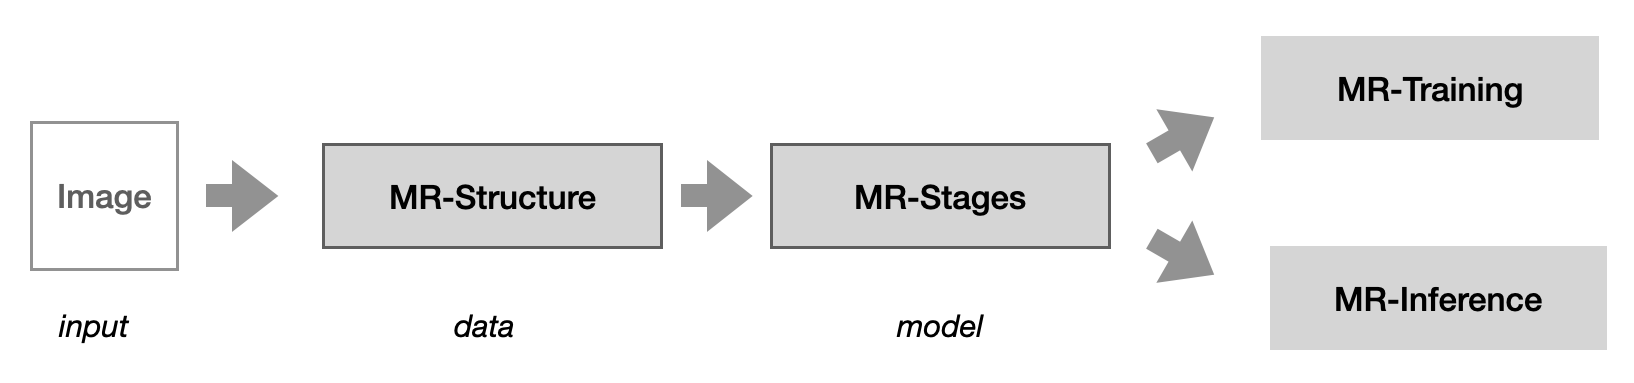
\includegraphics[width=0.99\linewidth]{img/ch4/mr-net-components.png}
% \caption{MR-Net framework Components.}
% \label{f:components}
% \end{figure}

% % Let $\gt{f}:\mathcal{D}\to \mathcal{C}$ be the ground-truth signal (\textit{input data}), and $f\!:\!\mathcal{D}\!\times\! [0,N]\!\to\! \mathcal{C}$ be a MR-Net with $N$ stages $\{g_i\}$ to fit $\gt{f}$~in multiresolution.
% % We use this setting to present the framework.

% \subsection{MR-Structure}\label{sec:mr_struct}

% The MR-Structure is a data structure that encapsulates the input data $\gt{f}$. It includes $\gt{f}$ and metadata about its \textit{sampling mode}, \textit{filtering type}, and the \textit{multi-stage stack} (see Fig~\ref{f:structure}).
% \begin{figure}[!h]
% \centering
% 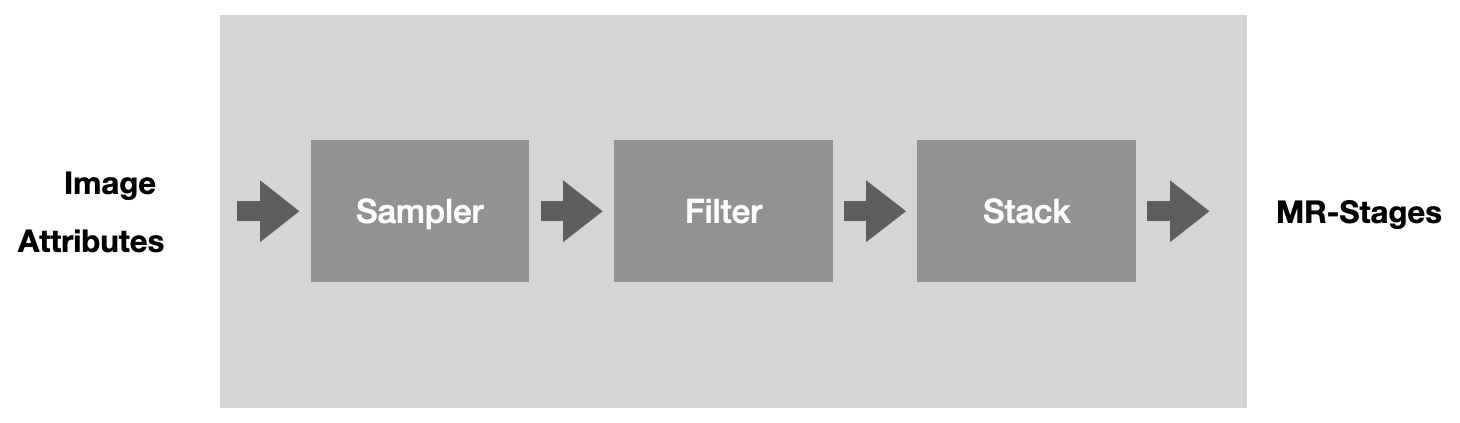
\includegraphics[width=0.89\linewidth]{img/ch4/mr-structure.png}
% \caption{MR-Structure.}
% \label{f:structure}
% \end{figure}

% For flexibility, we implement a sampler module that take regular samples or stochastic samples using the Poisson disk sampling~\cite{stochastic_cook, poisson_bridson}. 
% The sampler could be extended to work with different sampling patterns. 
% The sampling mode is stored in the MR-Structure, so it can be taken into account when doing operations that modify the sampling grid.

% \begin{figure}[!h]
% \centering
% 
\includegraphics[width=0.45\linewidth]{img/ch4/regular.png}
% \hfil
% 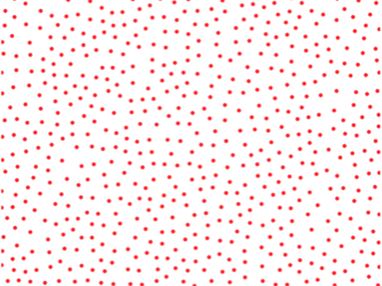
\includegraphics[width=0.45\linewidth]{img/ch4/poisson.png}
% \\
% {\small\hfil (regular grid) \hfil\hfil\hfil (irregular grid) \hfil}
% \caption{Sampling modes.}
% \label{f:sampling}
% \end{figure}

% % Nonetheless, it is also possible to define a irregular multiresolution grid structure. In this case, each resolution level has approximately twice the number of random sample points of the previous level .

% \subsection{Logger}

% The training of the MR-Net $f$ is monitored by a logging module that helps to visualize the learning progress. During training, the logger receives messages when the network training starts and ends, when a stage training starts and ends, when a epoch training ends, and when a batch training ends. 

% This architecture allows the logger to be customized to accommodate different MR-Net configurations and different actions for visualizing the training progress. For instance, it is possible to write a logger to save partial results to the disk, display~them in a development environment, or send them to a cloud based~service.



% \section{The Multiresolution Module}

% Our goal is to design a module capable of approximating a signal with multiple frequency bands. When we introduce hidden layers, we know, from previous experiments, that the model capacity increases and we can’t control the exact content of frequencies the network learns. This way, we aimed for a module with a single hidden layer and used Perlin Noises with 4 local extrema (Figure 17) as a perceptual indicator of ”limited frequency band”.

% We did experiments with 1 and 2 hidden layers modules using 8, 16 or 32 computational units in each layer. After looking at the results, we chose a module with 1 hidden layer and 16 units in each layer as our MR-Module for most experiments.

% \begin{figure}[h]
%     \centering
%     \begin{subfigure}[b]{0.3\textwidth}
%         \centering
%         
\includegraphics[width=\textwidth]{img/placeholder512.png}
%         % \caption{$Loss function$}
%         % \label{fig:diverging-loss}
%     \end{subfigure}
%     \begin{subfigure}[b]{0.3\textwidth}
%         \centering
%         
\includegraphics[width=\textwidth]{img/placeholder512.png}
%         % \caption{Reconstruction}
%         % \label{fig:diverging-reconstruction}
%     \end{subfigure}
%     \caption{Reconstruction of low frequency signals using a small size model}
%     % \label{f:mr-module}
% \end{figure}

% We have not targeted the minimal module possible, as Figure XXX shows this module is able to approximate more complex signals up to a certain frequency. Having a small module with reasonable capacity gives us more flexibility in terms of level of detail strategy and helps to keep each stage of different MR-Net architectures uniformly as we will discuss on the next section. However, the breadth and depth of the MR-Module could be adapted to specific applications without compromising compatibility with the MR-Nets architectures.